% generated from JIRA project LVV
% using template at /usr/share/miniconda/envs/docsteady-env/lib/python3.7/site-packages/docsteady/templates/tpr.latex.jinja2.
% using docsteady version 2.2.4
% Please do not edit -- update information in Jira instead
\documentclass[PSE,STR,toc]{lsstdoc}
\usepackage{geometry}
\usepackage{longtable,booktabs}
\usepackage{enumitem}
\usepackage{arydshln}
\usepackage{attachfile}
\usepackage{array}
\usepackage{dashrule}

\newcolumntype{L}[1]{>{\raggedright\let\newline\\\arraybackslash\hspace{0pt}}p{#1}}

\input meta.tex

\newcommand{\attachmentsUrl}{https://github.com/\gitorg/\lsstDocType-\lsstDocNum/blob/\gitref/attachments}
\providecommand{\tightlist}{
  \setlength{\itemsep}{0pt}\setlength{\parskip}{0pt}}

\setcounter{tocdepth}{4}

\begin{document}

\def\milestoneName{M2 Hexapod Functional Re-verification and Integration with SAL}
\def\milestoneId{}
\def\product{SIT-COM Integration}

\setDocCompact{true}

\title{LVV-P68: M2 Hexapod Functional Re-verification and Integration with SAL Test Plan and Report}
\setDocRef{\lsstDocType-\lsstDocNum}
\date{ 2022-05-04 }
\author{ Holger Drass }

% Most recent last
\setDocChangeRecord{
\addtohist{}{2020-02-20}{First Draft}{Kevin Siruno}
\addtohist{1.0}{2020-03-09}{LVV-P68 Approved \jira{SE-1372}.}{Kevin Siruno}
\addtohist{3.0}{2022-035-04}{M2 hexapod verification on level 3 report \jira{SITCOM-204}.}{Holger Drass}
\addtohist{3.1}{2022-035-04}{M2 hexapod verification on level 3 report after SE revision\jira{SITCOM-204}.}{Holger Drass}
}

\setDocCurator{Holger Drass}
\setDocUpstreamLocation{\url{https://github.com/lsst-dm/\lsstDocType-\lsstDocNum}}
\setDocUpstreamVersion{\vcsrevision}



\setDocAbstract{
This is the test plan and report for
\textbf{ M2 Hexapod Functional Re-verification and Integration with SAL},
an LSST milestone pertaining to the Project System Engineering and Commissioning.\\
This document is based on content automatically extracted from the Jira test database on \docDate.
The most recent change to the document repository was on \vcsDate.
}


\maketitle

\section{Introduction}
\label{sect:intro}


\subsection{Objectives}
\label{sect:objectives}

 The objective of this test plan is to re-verify

\begin{itemize}
\tightlist
\item
  the hardware and software functional requirements of the M2 hexapod
  without SAL
\item
  the software functional requirements of the M2 hexapod integrated with
  SAL 4.0 or higher.
\end{itemize}

This re-verification is done after shipment from the vendor's facility
to the Summit, as defined in \citeds{LTS-206} and \citeds{LTS-160}.\\
This test campaign will exercise the functionality of the hardware and
software that was executed previously and meets the following criteria:

\begin{itemize}
\tightlist
\item
  Requires a laser tracker, mechanical gauges, induction current probe,
  temperature sensors
\item
  Requires the vendor's EUI software and hardware via local control
\item
  Requires control via SAL 4.0 or higher
\end{itemize}

The hardware and software requirements were previously verified during
the test campaign by the vendor at the vendor's facility and accepted by
LSST during the Factory Acceptance Test review.



\subsection{System Overview}
\label{sect:systemoverview}

 The purpose of the M2 hexapod is to maintain proper orientation of the
M2 Cell Assembly. It is attached to the spider spindle of the Top End
Assembly of the TMA. Although the mass of the M2 mirror cell assembly is
greater than the camera, the actuators of the M2 hexapod are identical
to the Camera Hexapod's actuators. For this reason, the M2 Hexapod and
Camera hexapod have the same operator's manual and similar test
procedures.~


\subsection{Document Overview}
\label{sect:docoverview}

This document was generated from Jira, obtaining the relevant information from the
\href{https://jira.lsstcorp.org/secure/Tests.jspa\#/testPlan/LVV-P68}{LVV-P68}
~Jira Test Plan and related Test Cycles (
\href{https://jira.lsstcorp.org/secure/Tests.jspa\#/testCycle/LVV-C147}{LVV-C147}
\href{https://jira.lsstcorp.org/secure/Tests.jspa\#/testCycle/LVV-C203}{LVV-C203}
).

Section \ref{sect:intro} provides an overview of the test campaign, the system under test (\product{}),
the applicable documentation, and explains how this document is organized.
Section \ref{sect:testplan} provides additional information about the test plan, like for example the configuration
used for this test or related documentation.
Section \ref{sect:personnel} describes the necessary roles and lists the individuals assigned to them.

Section \ref{sect:overview} provides a summary of the test results, including an overview in Table \ref{table:summary},
an overall assessment statement and suggestions for possible improvements.
Section \ref{sect:detailedtestresults} provides detailed results for each step in each test case.

The current status of test plan \href{https://jira.lsstcorp.org/secure/Tests.jspa\#/testPlan/LVV-P68}{LVV-P68} in Jira is \textbf{ Approved }.

\subsection{References}
\label{sect:references}
\renewcommand{\refname}{}
\bibliography{lsst,refs,books,refs_ads,local}


\newpage
\section{Test Plan Details}
\label{sect:testplan}


\subsection{Data Collection}

  Observing is not required for this test campaign.

\subsection{Verification Environment}
\label{sect:hwconf}
  This test plan is going to be executed in two verification environments:

\begin{itemize}
\tightlist
\item
  The M2 Hexapod will be verified in a climate-controlled environment
  \textbf{on the 3rd floor of the Summit Facility} on the TEA structure
  with \textbf{the M2 mass surrogate installed and facing downwards.}
  The TEA is mounted on its shipping mount.
\item
  The M2 Hexapod will be verified \textbf{on the TMA in the Dome of the
  Summit Facility} on the TEA structure with \textbf{the M2 mass
  surrogate installed and following the elevation suggested in the
  vendor's documentation.\\
  }
\end{itemize}

  \subsection{Entry Criteria}
  In order to test the M2 Hexapod functionality, the following criteria
must be met first:

\begin{itemize}
\tightlist
\item
  All the test setup for the Data Acquisition system must be completed
  and ready to record data for the laser tracker
\item
  The laser tracker and 3 SMRs are installed and setup
\item
  All utilities and electrical connections are hooked up and allow the
  M2 Hexapod to be powered on and controlled
\item
  The EFD must be set up to be able to store events and telemetry data
\item
  The temperature measurement system is operational and the EFD is able
  to record temperature
\end{itemize}

  \subsection{Exit Criteria}
  In order for this event to be considered complete, the following
criteria must be met:

\begin{itemize}
\tightlist
\item
  Raw test data, events, and telemetry have been saved for the M2
  Hexapod in the EFD.
\item
  All test data has been analyzed and post-processed.
\item
  All test steps have been statused in the Jira Test Cases within this
  Test Plan and actual results populated as required.
\item
  A summary of the results of the test campaign has been captured in the
  Overall Assessment and Recommended Improvements fields of this Test
  Plan
\item
  A link to the verification artifacts used to produce the summary of
  results has been populated in the Verification Artifacts field of this
  Test Plan
\item
  For tests producing quantitative results reporting of the analysis
  shall include traceability to the raw data of the test and estimates
  for the statistical significance of the result(s).
\item
  Any failures have been captured in the
  \href{https://jira.lsstcorp.org/projects/FRACAS/issues/}{FRACAS}
  project
\end{itemize}


\subsection{Related Documentation}


No additional documentation provided.


\subsection{PMCS Activity}

Primavera milestones related to the test campaign:
\begin{itemize}
\item None
\end{itemize}


\newpage
\section{Personnel}
\label{sect:personnel}

The personnel involved in the test campaign is shown in the following table.

{\small
\begin{longtable}{p{3cm}p{3cm}p{3cm}p{6cm}}
\hline
\multicolumn{2}{r}{T. Plan \href{https://jira.lsstcorp.org/secure/Tests.jspa\#/testPlan/LVV-P68}{LVV-P68} owner:} &
\multicolumn{2}{l}{\textbf{ Holger Drass } }\\\hline
\multicolumn{2}{r}{T. Cycle \href{https://jira.lsstcorp.org/secure/Tests.jspa\#/testCycle/LVV-C147}{LVV-C147} owner:} &
\multicolumn{2}{l}{\textbf{
Holger Drass }
} \\\hline
\textbf{Test Cases} & \textbf{Assigned to} & \textbf{Executed by} & \textbf{Additional Test Personnel} \\ \hline
\href{https://jira.lsstcorp.org/secure/Tests.jspa#/testCase/LVV-T1804}{LVV-T1804}
& {\small Holger Drass } & {\small Holger Drass } &
\begin{minipage}[]{6cm}
\smallskip
{\small (1) Software Engineer\\
(1) Hardware Engineer }
\medskip
\end{minipage}
\\ \hline
\href{https://jira.lsstcorp.org/secure/Tests.jspa#/testCase/LVV-T1800}{LVV-T1800}
& {\small Holger Drass } & {\small Holger Drass } &
\begin{minipage}[]{6cm}
\smallskip
{\small (1) Software Engineer\\
(1) Mechanical Engineer\\
(1) Systems Engineer\\[2\baselineskip] }
\medskip
\end{minipage}
\\ \hline
\href{https://jira.lsstcorp.org/secure/Tests.jspa#/testCase/LVV-T1802}{LVV-T1802}
& {\small Holger Drass } & {\small Holger Drass } &
\begin{minipage}[]{6cm}
\smallskip
{\small (1) Software Engineer\\
(1) Hardware Engineer }
\medskip
\end{minipage}
\\ \hline
\multicolumn{2}{r}{T. Cycle \href{https://jira.lsstcorp.org/secure/Tests.jspa\#/testCycle/LVV-C203}{LVV-C203} owner:} &
\multicolumn{2}{l}{\textbf{
Holger Drass }
} \\\hline
\textbf{Test Cases} & \textbf{Assigned to} & \textbf{Executed by} & \textbf{Additional Test Personnel} \\ \hline
\end{longtable}
}

\newpage

\section{Test Campaign Overview}
\label{sect:overview}

\subsection{Summary}
\label{sect:summarytable}

{\small
\begin{longtable}{p{2cm}cp{2.3cm}p{8.6cm}p{2.3cm}}
\toprule
\multicolumn{2}{r}{ T. Plan \href{https://jira.lsstcorp.org/secure/Tests.jspa\#/testPlan/LVV-P68}{LVV-P68}:} &
\multicolumn{2}{p{10.9cm}}{\textbf{ M2 Hexapod Functional Re-verification and Integration with SAL }} & Approved \\\hline
\multicolumn{2}{r}{ T. Cycle \href{https://jira.lsstcorp.org/secure/Tests.jspa\#/testCycle/LVV-C147}{LVV-C147}:} &
\multicolumn{2}{p{10.9cm}}{\textbf{ M2 Hexapod Re-verification on Level 3 }} & Done \\\hline
\textbf{Test Cases} &  \textbf{Ver.} & \textbf{Status} & \textbf{Comment} & \textbf{Issues} \\\toprule
\href{https://jira.lsstcorp.org/secure/Tests.jspa#/testCase/LVV-T1804}{LVV-T1804}
&  1
& Initial Pass &
\begin{minipage}[]{9cm}
\smallskip
The start-up procedure was executed in a different test case before and
did not need to be executed again.
\medskip
\end{minipage}
&   \\\hline
\href{https://jira.lsstcorp.org/secure/Tests.jspa#/testCase/LVV-T1800}{LVV-T1800}
&  1
& Fail &
\begin{minipage}[]{9cm}
\smallskip
Since this execution, this (M2) hexapod was lifted to the TMA. ~In the
meantime, the \textbf{camera~}hexapod software and hardware were
extensively tested and improved.\\[2\baselineskip]
\medskip
\end{minipage}
&   \href{https://jira.lsstcorp.org/browse/LVV-19511}{LVV-19511}
\href{https://jira.lsstcorp.org/browse/LVV-19511}{LVV-19511}
\href{https://jira.lsstcorp.org/browse/LVV-19511}{LVV-19511}
\href{https://jira.lsstcorp.org/browse/LVV-19511}{LVV-19511}
\\\hline
\href{https://jira.lsstcorp.org/secure/Tests.jspa#/testCase/LVV-T1802}{LVV-T1802}
&  2
& Fail &
\begin{minipage}[]{9cm}
\smallskip

\medskip
\end{minipage}
&   \href{https://jira.lsstcorp.org/browse/LVV-19512}{LVV-19512}
\href{https://jira.lsstcorp.org/browse/LVV-19512}{LVV-19512}
\href{https://jira.lsstcorp.org/browse/LVV-19512}{LVV-19512}
\href{https://jira.lsstcorp.org/browse/LVV-19512}{LVV-19512}
\href{https://jira.lsstcorp.org/browse/LVV-19512}{LVV-19512}
\href{https://jira.lsstcorp.org/browse/LVV-19512}{LVV-19512}
\href{https://jira.lsstcorp.org/browse/LVV-19512}{LVV-19512}
\href{https://jira.lsstcorp.org/browse/LVV-19512}{LVV-19512}
\\\hline
\multicolumn{2}{r}{ T. Cycle \href{https://jira.lsstcorp.org/secure/Tests.jspa\#/testCycle/LVV-C203}{LVV-C203}:} &
\multicolumn{2}{p{10.9cm}}{\textbf{ M2 Hexapod Re-verification on the TMA }} & Not Executed \\\hline
\textbf{Test Cases} &  \textbf{Ver.} & \textbf{Status} & \textbf{Comment} & \textbf{Issues} \\\toprule
\caption{Test Campaign Summary}
\label{table:summary}
\end{longtable}
}

\subsection{Overall Assessment}
\label{sect:overallassessment}

\textbf{The following results are for the first
test-cycle~\href{https://jira.lsstcorp.org/secure/Tests.jspa\#/testCycle/LVV-C147}{LVV-C147}:}\\
During the February 2020 verification, the M2 hexapod was still on level
three, and the M2 hexapod software components low-level controller, EUI,
and CSC were still under development.\\
Since the hexapod has been received from the vendor the sets of commands
for the EUI and the CSC have diverged. The ``positionSet'' command is
only supported by the EUI and is retired for the CSC. At the CSC level,
this functionality is now included directly in the commands to move the
hexapod. Other commands were either modified themselves or their payload
has changed. For an up-to-date list of all supported commands and their
permitted payloads see
\href{https://ts-xml.lsst.io/sal_interfaces/MTHexapod.html}{MT Hexapod
Sal interfaces}.\\
Some events were not created in the EFD as expected. In detail, the
``inPosition'' and ``controlledStop'' events were not generated in the
EFD. The ``compensationMode'' was not activating correctly and not
reported to the EFD as expected. For details see the
\href{https://jira.lsstcorp.org/secure/Tests.jspa\#/testPlayer/testExecution/LVV-E1028}{Execution
of test case LVV-T1804} and the
\href{https://jira.lsstcorp.org/secure/Tests.jspa\#/testPlayer/testExecution/LVV-E1021}{execution
of test case LVV-T1802}.\\
Apart from this, the CSC is going to be updated to a standbyState-entry
state machine. This implies that the start-up procedure will change.
Various other changes were necessary to keep up with the development of
the SAL/DDS itself and to accommodate changes in the network
infrastructure of the observatory.\\
All of these changes have been tested with positive results using the
camera hexapod since the M2 hexapod was lifted on top of the TMA and is
not accessible for a long time.\\[2\baselineskip]On the hardware side,
the M2 hexapod presented random faults in Drive 0 and Drive 1. The
failure is randomly happening over a time range between a few minutes
and at least 11 hours. The fault appears in the EFD and on the EUI. On
the EUI the fault is presented as ``Feedback Error Drive0''. A detailed
investigation on this issue was performed by first switching the cables
to a different actuator and later by changing the actuator itself. Both
attempts are excluding that an actuator as the source of failure but did
not solve the problem (for details see
\href{https://jira.lsstcorp.org/browse/FRACAS-53}{FRACAS-53}). This
issue was also observed on the camera hexapod and was solved by changing
the cables to the actuators.\\
The second hardware-related issue concerns the requirements
\href{https://jira.lsstcorp.org/browse/LVV-18622}{LTS-206-REQ-0164-V-02:
3.5.12\_1 Positioning - LSST Re-verification} and
\href{https://jira.lsstcorp.org/browse/LVV-18631}{LTS-206-REQ-0178-V-02:
3.5.24\_1 Hexapod Absolute Accuracy - LSST Re-verification}. Tests on
the positioning in X,Y,Z translation combined with a rotation failed to
reach the required precision. The same issue was observed for the
hexapod's absolute accuracy. The reasons are lying most likely in the
measurement setup itself. The laser tracker measurements are at the
limit of the laser tracker's precision and the Mitutoyo gauges mounts
were a preliminary solution. Testing the camera hexapod with an improved
Mitutoyo setup has shown that the same requirements are fulfilled for
the camera hexapod. The hardware tests are executed and documented as
part of the
\href{https://jira.lsstcorp.org/secure/Tests.jspa\#/testPlayer/testExecution/LVV-E1022}{execution
of test case LVV-T1800}.\\
In addition, all the aforementioned tests and discoveries were done
shortly before the M2 hexapod needed to be installed at the TMA.
Therefore, some of the hardware tests could not be
executed.\\[2\baselineskip]\textbf{The following results are for the
second test cycle:}\\[3\baselineskip]

\subsection{Recommended Improvements}
\label{sect:recommendations}

\textbf{The following recommendations are derived from the first
test-cycle}\\
As a general comment, enough time should be allocated to test the EUI
and CSC commands as well as to execute the rest of the hardware tests.\\
To improve the situation before the tests on the TMA the recommendation
is to update the M2 hexapod low-level controller, the EUI, and the CSC
to the latest versions.\\
The software tests for the EUI should be executed when the state machine
is updated to the standbyState-entry state machine. The test case should
be updated to account for state machine tests.\\
The configuration part of the test cases should be updated to account
for the change in accordance with \citeds{LSE-209} and need to be tested for the
first time.\\
For the hardware aspects of the M2 hexapod, a new measurement setup that
is similar to what was used for the camera hexapod should be used. With
the new measurement setup in place, the failing tests should be repeated
to confirm the positioning in X,Y,Z in combination with rotation and the
hexapod's absolute accuracy are within their requirements
(\href{https://jira.lsstcorp.org/browse/LVV-18622}{LTS-206-REQ-0164-V-02:
3.5.12\_1 Positioning - LSST Re-verification} and
\href{https://jira.lsstcorp.org/browse/LVV-18631}{LTS-206-REQ-0178-V-02:
3.5.24\_1 Hexapod Absolute Accuracy - LSST Re-verification}). In case
new faults are encountered, especially blind spots on the encoders,
cleaning of the actuators similar to the camera hexapod actuators should
be performed. To address the random fault in drive zero and to ensure
that is not happening in another drive all the cables for the M2 hexapod
should be updated similar to the camera hexapod and the 32 MOOG test
moves (Moog test protocol paragraph 3.5.12), as well as the endurance
test corresponding to one night of operation, should be executed. The
\href{https://jira.lsstcorp.org/browse/FRACAS-53}{FRACAS-53} ticket
should be closed out.\\[2\baselineskip]Test cases with an ``initial
pass'' or ``fail'' need to be executed in the next test cycle. The test
plan needs to be revised, and make a new test cycle with the M2 hexapod
on the TMA. Update the test cases to include the updated software and
updated wiring and the improved gauge measurement setup. All of the
``Not executed'' steps need to be revised as required and executed
because we did not have enough time to execute the
tests.\\[2\baselineskip]\textbf{The following recommendations are
derived from the second test-cycle:}

\newpage
\section{Detailed Test Results}
\label{sect:detailedtestresults}

\subsection{Test Cycle LVV-C147 }

Open test cycle {\it \href{https://jira.lsstcorp.org/secure/Tests.jspa#/testrun/LVV-C147}{M2 Hexapod Re-verification on Level 3}} in Jira.

Test Cycle name: M2 Hexapod Re-verification on Level 3\\
Status: Done

Re-verify the hardware and software for the M2 Hexapod that was
previously tested by MOOG and verify the integrated M2 hexapod with SAL
4.0 or higher.

\subsubsection{Software Version/Baseline}
\begin{enumerate}
\tightlist
\item
  M2 Hexapod Control Software with SAL v4.0 or higher
\item
  EFD with SAL v4.0 or higher
\end{enumerate}

\subsubsection{Configuration}
No varying configuration between test cycles.

\subsubsection{Test Cases in LVV-C147 Test Cycle}

\paragraph{ LVV-T1804 - M2 Hexapod Software Functional Re-verification }\mbox{}\\

Version \textbf{1}.
Open  \href{https://jira.lsstcorp.org/secure/Tests.jspa#/testCase/LVV-T1804}{\textit{ LVV-T1804 } }
test case in Jira.

The objective of this test case is to re-verify the functional
requirements of the M2 hexapod's software, after shipment of the
hardware from the vendor's facility to the Summit, as defined in \citeds{LTS-206}
and \citeds{LTS-160}. This test case will only exercise the functionality that
was executed previously and meets the following criteria:

\begin{itemize}
\tightlist
\item
  Only requires the M2 hexapod to be operable
\item
  Only requires testing the synchronous mode

  \begin{itemize}
  \tightlist
  \item
    \textbf{Asynchronous mode is not a standard mode of operation}
  \end{itemize}
\item
  Only requires the vendor's EUI software and hardware via local control

  \begin{itemize}
  \tightlist
  \item
    Does \textbf{NOT} require integration with SAL
  \end{itemize}
\item
  Does \textbf{NOT} require the M2 hexapod to be rotated to various
  elevation angles.
\item
  This test case can be executed with a \textbf{simulated M2 mass or
  actual M2 hardware}
\end{itemize}

The software functional requirements were previously verified during the
test campaign by the vendor at the vendor's facility and accepted by
Rubin Observatory during the Factory Acceptance Test review. The test
procedure used during the vendor's acceptance testing is the \emph{LSST
Hexapods-Rotator Software Acceptance Test Procedure} which is attached
to this test case. The test steps of this test case are taken directly
from that document on how to perform the test in a similar way as was
performed previously and the test steps include changes noted by the
vendor.\\[2\baselineskip]See the attached \emph{LSST Hexapod Operator's
Manual} for more information on how to operate the hexapod.

\textbf{ Preconditions}:\\
Prior to the execution of this test case to re-verify the M2 Hexapod
hardware functional requirements, the following Summit tasks must be
completed:

\begin{itemize}
\tightlist
\item
  The measurement equipment has been set up for testing

  \begin{itemize}
  \tightlist
  \item
    \url{https://jira.lsstcorp.org/browse/SUMMIT-1943}
  \end{itemize}
\end{itemize}

Execution status: {\bf Initial Pass }

Final comment:\\The start-up procedure was executed in a different test case before and
did not need to be executed again.


Detailed steps results:

\begin{tabular}{p{2cm}p{14cm}}
\toprule
Step 1 & Step Execution Status: \textbf{ Pass } \\ \hline
\end{tabular}
 Description \\
{\footnotesize
\textbf{STARTING THE EUI}\\[2\baselineskip]Double click the Hexapod GUI
Viewer desktop icon on the computer.

\begin{itemize}
\tightlist
\item
  This can be done on the Dell Management PC or another computer on the
  same network
\end{itemize}

}
\hdashrule[0.5ex]{\textwidth}{1pt}{3mm}
  Expected Result \\
{\footnotesize
A prompt to enter the password is shown.

}
\hdashrule[0.5ex]{\textwidth}{1pt}{3mm}
  Actual Result \\
{\footnotesize
\textbf{Deviation:}

\begin{itemize}
\tightlist
\item
  Access is now through X2GO.
\end{itemize}

}
\begin{tabular}{p{2cm}p{14cm}}
\toprule
Step 2 & Step Execution Status: \textbf{ Pass } \\ \hline
\end{tabular}
 Description \\
{\footnotesize
Enter the password ``lsst-vnc''

\begin{itemize}
\tightlist
\item
  If the EUI isn't automatically up and running when the VNC opens,
  double click on the Hexapod-eGUI icon on the VNC viewer
\end{itemize}

}
\hdashrule[0.5ex]{\textwidth}{1pt}{3mm}
  Expected Result \\
{\footnotesize
The EUI is in the Offline State/PublishOnly substate and is able to
publish through SAL but cannot receive commands.

}
\hdashrule[0.5ex]{\textwidth}{1pt}{3mm}
  Actual Result \\
{\footnotesize
\textbf{Deviation:}

\begin{itemize}
\tightlist
\item
  Access is now through X2GO.
\item
  Use the command line to start the latest version of the EUI.
\item
  Starts in Offline State/PublishOnly.
\end{itemize}

}
\begin{tabular}{p{2cm}p{14cm}}
\toprule
Step 3 & Step Execution Status: \textbf{ Initial Pass } \\ \hline
\end{tabular}
 Description \\
{\footnotesize
\textbf{OFFLINESTATE/AVAILABLESTATE}\\
On the Main tab, select the ``Offline SubState Cmd'' field in the
Commands to Send section, set the Offline SubState Triggers to ``System
Ready'' and click on the Send Command button.\\
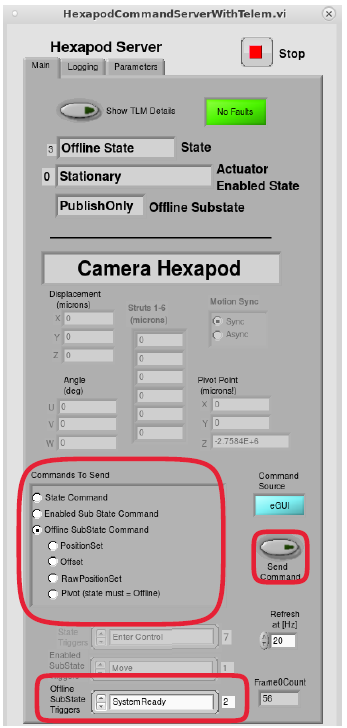
\includegraphics[width=1.79167in]{jira_imgs/1024.png}

}
\hdashrule[0.5ex]{\textwidth}{1pt}{3mm}
  Expected Result \\
{\footnotesize
The system transitions from the OfflineState/PublishOnly substate to the
OfflineState/AvailableState substate and the Command Source says
eGUI.\\[2\baselineskip]

}
\hdashrule[0.5ex]{\textwidth}{1pt}{3mm}
  Actual Result \\
{\footnotesize

}
\begin{tabular}{p{2cm}p{14cm}}
\toprule
Step 4 & Step Execution Status: \textbf{ Initial Pass } \\ \hline
\end{tabular}
 Description \\
{\footnotesize
\textbf{OFFLINESTATE -\textgreater{} STANDBYSTATE}\\
Click on the State Command field in the Commands to Send section.\\
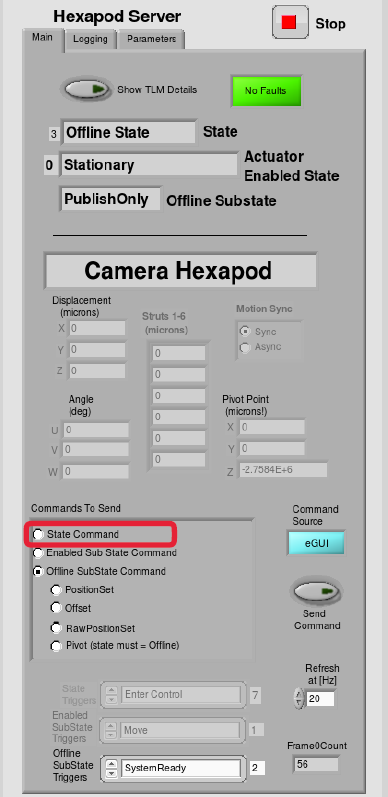
\includegraphics[width=1.79167in]{jira_imgs/1028.png}

}
\hdashrule[0.5ex]{\textwidth}{1pt}{3mm}
  Expected Result \\
{\footnotesize
The State Triggers dialogue box shown below becomes visible.\\
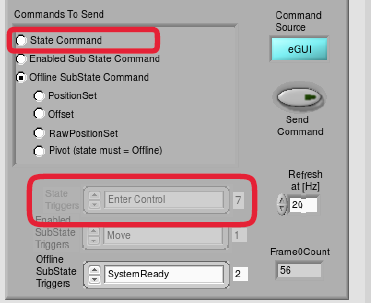
\includegraphics[width=1.79167in]{jira_imgs/1029.png}

}
\hdashrule[0.5ex]{\textwidth}{1pt}{3mm}
  Actual Result \\
{\footnotesize

}
\begin{tabular}{p{2cm}p{14cm}}
\toprule
Step 5 & Step Execution Status: \textbf{ Initial Pass } \\ \hline
\end{tabular}
 Description \\
{\footnotesize
Scroll through the available trigger options to select ``Enter Control''
and click the Send Command button.

}
\hdashrule[0.5ex]{\textwidth}{1pt}{3mm}
  Expected Result \\
{\footnotesize
The system transitions to the Standby state and the primary state
display box at the top of the Main says Standby State.

}
\hdashrule[0.5ex]{\textwidth}{1pt}{3mm}
  Actual Result \\
{\footnotesize

}
\begin{tabular}{p{2cm}p{14cm}}
\toprule
Step 6 & Step Execution Status: \textbf{ Initial Pass } \\ \hline
\end{tabular}
 Description \\
{\footnotesize
\textbf{STANDBYSTATE -\textgreater{} DISABLEDSTATE}\\
From the StandbyState, send a Start State command.

}
\hdashrule[0.5ex]{\textwidth}{1pt}{3mm}
  Expected Result \\
{\footnotesize
The system transitions into DisabledState and the current configuration
parameters are maintained from the default parameters or from the
previous DDS start command.~

}
\hdashrule[0.5ex]{\textwidth}{1pt}{3mm}
  Actual Result \\
{\footnotesize

}
\begin{tabular}{p{2cm}p{14cm}}
\toprule
Step 7 & Step Execution Status: \textbf{ Initial Pass } \\ \hline
\end{tabular}
 Description \\
{\footnotesize
\textbf{DISABLEDSTATE -\textgreater{} ENABLEDSTATE}\\
From the DisabledState, send an Enable State Command.~

}
\hdashrule[0.5ex]{\textwidth}{1pt}{3mm}
  Expected Result \\
{\footnotesize
The system transitions into the EnabledState/Stationary substate, the
motor drives are enabled and and motion can be commanded.~

}
\hdashrule[0.5ex]{\textwidth}{1pt}{3mm}
  Actual Result \\
{\footnotesize

}
\begin{tabular}{p{2cm}p{14cm}}
\toprule
Step 8 & Step Execution Status: \textbf{ Not Executed } \\ \hline
\end{tabular}
 Description \\
{\footnotesize
\textless{}conditional state\textgreater{}\\
\textbf{FAULTSTATE}\\
If a Fault occurs in any of the other states, the system will
automatically transition to the Fault State. While in the Fault state,
send a clearError.\\
Note: If the fault that occurs goes through the interlock system, reset
the safety relay switch and send a clearError command.

}
\hdashrule[0.5ex]{\textwidth}{1pt}{3mm}
  Expected Result \\
{\footnotesize
The system transitions back to the OfflineState/PublishOnly substate.
(Go back to Step 3)

}
\hdashrule[0.5ex]{\textwidth}{1pt}{3mm}
  Actual Result \\
{\footnotesize

}
\begin{tabular}{p{2cm}p{14cm}}
\toprule
Step 9 & Step Execution Status: \textbf{ Initial Pass } \\ \hline
\end{tabular}
 Description \\
{\footnotesize
\textbf{Section 3.3.1 EUI Tests of the attached Software Acceptance Test
Procedure}\\
At startup, confirm that the system starts in the Offline/PublishOnly
state.

}
\hdashrule[0.5ex]{\textwidth}{1pt}{3mm}
  Expected Result \\
{\footnotesize
The hexapod starts in the Offline/PublishOnly state.

}
\hdashrule[0.5ex]{\textwidth}{1pt}{3mm}
  Actual Result \\
{\footnotesize
The state machine in general allowed to transition the M2 hexapod in the
enabledState/Stationary and to clear faults when necessary. The state
machine was under development during this testing period not further
investigated.

}
\begin{tabular}{p{2cm}p{14cm}}
\toprule
Step 10 & Step Execution Status: \textbf{ Not Executed } \\ \hline
\end{tabular}
 Description \\
{\footnotesize
Send an offline substate trigger of systemReady.

}
\hdashrule[0.5ex]{\textwidth}{1pt}{3mm}
  Expected Result \\
{\footnotesize
The system transitions into the Offline/Available substate.

}
\hdashrule[0.5ex]{\textwidth}{1pt}{3mm}
  Actual Result \\
{\footnotesize

}
\begin{tabular}{p{2cm}p{14cm}}
\toprule
Step 11 & Step Execution Status: \textbf{ Not Executed } \\ \hline
\end{tabular}
 Description \\
{\footnotesize
Send an EnterControl trigger.

}
\hdashrule[0.5ex]{\textwidth}{1pt}{3mm}
  Expected Result \\
{\footnotesize
The system transitions from Offline/Available to Standby state.

}
\hdashrule[0.5ex]{\textwidth}{1pt}{3mm}
  Actual Result \\
{\footnotesize

}
\begin{tabular}{p{2cm}p{14cm}}
\toprule
Step 12 & Step Execution Status: \textbf{ Not Executed } \\ \hline
\end{tabular}
 Description \\
{\footnotesize
Send a Start trigger.

}
\hdashrule[0.5ex]{\textwidth}{1pt}{3mm}
  Expected Result \\
{\footnotesize
The system transitions from Standby to Disabled state.

}
\hdashrule[0.5ex]{\textwidth}{1pt}{3mm}
  Actual Result \\
{\footnotesize

}
\begin{tabular}{p{2cm}p{14cm}}
\toprule
Step 13 & Step Execution Status: \textbf{ Not Executed } \\ \hline
\end{tabular}
 Description \\
{\footnotesize
Send an Enable trigger.

}
\hdashrule[0.5ex]{\textwidth}{1pt}{3mm}
  Expected Result \\
{\footnotesize
The system transitions from Disabled to Enabled state.

}
\hdashrule[0.5ex]{\textwidth}{1pt}{3mm}
  Actual Result \\
{\footnotesize

}
\begin{tabular}{p{2cm}p{14cm}}
\toprule
Step 14 & Step Execution Status: \textbf{ Not Executed } \\ \hline
\end{tabular}
 Description \\
{\footnotesize
Send a Disable trigger.

}
\hdashrule[0.5ex]{\textwidth}{1pt}{3mm}
  Expected Result \\
{\footnotesize
The system transitions from Enabled to Disabled state.

}
\hdashrule[0.5ex]{\textwidth}{1pt}{3mm}
  Actual Result \\
{\footnotesize

}
\begin{tabular}{p{2cm}p{14cm}}
\toprule
Step 15 & Step Execution Status: \textbf{ Not Executed } \\ \hline
\end{tabular}
 Description \\
{\footnotesize
Send a Standby trigger.

}
\hdashrule[0.5ex]{\textwidth}{1pt}{3mm}
  Expected Result \\
{\footnotesize
The system transitions from Disabled state to Standby state.

}
\hdashrule[0.5ex]{\textwidth}{1pt}{3mm}
  Actual Result \\
{\footnotesize

}
\begin{tabular}{p{2cm}p{14cm}}
\toprule
Step 16 & Step Execution Status: \textbf{ Not Executed } \\ \hline
\end{tabular}
 Description \\
{\footnotesize
Send a exitControl trigger.

}
\hdashrule[0.5ex]{\textwidth}{1pt}{3mm}
  Expected Result \\
{\footnotesize
The system transitions from Standby state to Offline state.

}
\hdashrule[0.5ex]{\textwidth}{1pt}{3mm}
  Actual Result \\
{\footnotesize

}
\begin{tabular}{p{2cm}p{14cm}}
\toprule
Step 17 & Step Execution Status: \textbf{ Not Executed } \\ \hline
\end{tabular}
 Description \\
{\footnotesize
Return to the Enabled state and trip the safety interlock switch.

}
\hdashrule[0.5ex]{\textwidth}{1pt}{3mm}
  Expected Result \\
{\footnotesize
The system transitions to Fault state.

}
\hdashrule[0.5ex]{\textwidth}{1pt}{3mm}
  Actual Result \\
{\footnotesize

}
\begin{tabular}{p{2cm}p{14cm}}
\toprule
Step 18 & Step Execution Status: \textbf{ Initial Pass } \\ \hline
\end{tabular}
 Description \\
{\footnotesize
Reset the safety interlock and send a ClearError trigger.

}
\hdashrule[0.5ex]{\textwidth}{1pt}{3mm}
  Expected Result \\
{\footnotesize
The CSC, upon receiving the ¨clearError¨ trigger, transitions from
FaultState to OfflineState/PublishOnly when the system was in any of the
OfflineStates before the error occurred. The CSC, upon receiving the
``clearError'' trigger, transitions to StandbyState when it was in
EnableState or DisableState before the error occurred.

}
\hdashrule[0.5ex]{\textwidth}{1pt}{3mm}
  Actual Result \\
{\footnotesize

}
\begin{tabular}{p{2cm}p{14cm}}
\toprule
Step 19 & Step Execution Status: \textbf{ Not Executed } \\ \hline
\end{tabular}
 Description \\
{\footnotesize
\textbf{Section 4.1 Hexapod Events of the attached Software Acceptance
Test Procedure}\\[2\baselineskip]In the Enabled/Stationary state, unplug
a motor encoder cable for one of the actuators.

}
\hdashrule[0.5ex]{\textwidth}{1pt}{3mm}
  Test Data \\
 {\footnotesize
\textbf{Deviation:~}Perform the following set of steps using the EUI
instead of the DDS and verify the events are displayed on the EUI.

}
\hdashrule[0.5ex]{\textwidth}{1pt}{3mm}
  Expected Result \\
{\footnotesize
A Drive Fault error event is created and the system transitions to Fault
state.

}
\hdashrule[0.5ex]{\textwidth}{1pt}{3mm}
  Actual Result \\
{\footnotesize
Not tested

}
\begin{tabular}{p{2cm}p{14cm}}
\toprule
Step 20 & Step Execution Status: \textbf{ Not Executed } \\ \hline
\end{tabular}
 Description \\
{\footnotesize
Send the ``clearError'' trigger and bring the system to the
Enabled/Stationary state.

}
\hdashrule[0.5ex]{\textwidth}{1pt}{3mm}
  Expected Result \\
{\footnotesize
The system is in the Enabled/Stationary state and ready to be commanded.

}
\hdashrule[0.5ex]{\textwidth}{1pt}{3mm}
  Actual Result \\
{\footnotesize

}
\begin{tabular}{p{2cm}p{14cm}}
\toprule
Step 21 & Step Execution Status: \textbf{ Not Executed } \\ \hline
\end{tabular}
 Description \\
{\footnotesize
In the Enabled/Stationary state, unplug a linear encoder cable for one
of the actuators.~

}
\hdashrule[0.5ex]{\textwidth}{1pt}{3mm}
  Expected Result \\
{\footnotesize
A Drive Fault error event is created and the system transitions to Fault
state.

}
\hdashrule[0.5ex]{\textwidth}{1pt}{3mm}
  Actual Result \\
{\footnotesize
Not tested

}
\begin{tabular}{p{2cm}p{14cm}}
\toprule
Step 22 & Step Execution Status: \textbf{ Not Executed } \\ \hline
\end{tabular}
 Description \\
{\footnotesize
Send the ``clearError'' trigger and bring the system to the
Enabled/Stationary state.

}
\hdashrule[0.5ex]{\textwidth}{1pt}{3mm}
  Expected Result \\
{\footnotesize
The system is in the Enabled/Stationary state and ready to be commanded.

}
\hdashrule[0.5ex]{\textwidth}{1pt}{3mm}
  Actual Result \\
{\footnotesize

}
\begin{tabular}{p{2cm}p{14cm}}
\toprule
Step 23 & Step Execution Status: \textbf{ Not Executed } \\ \hline
\end{tabular}
 Description \\
{\footnotesize
Unplug a motor power cable from one of the actuators and command a
PositionSet/Move.~

}
\hdashrule[0.5ex]{\textwidth}{1pt}{3mm}
  Expected Result \\
{\footnotesize
A Following Error event is created and the system transitions to Fault
state.

}
\hdashrule[0.5ex]{\textwidth}{1pt}{3mm}
  Actual Result \\
{\footnotesize
not tested

}
\begin{tabular}{p{2cm}p{14cm}}
\toprule
Step 24 & Step Execution Status: \textbf{ Not Executed } \\ \hline
\end{tabular}
 Description \\
{\footnotesize
Send the ``clearError'' trigger and bring the system to the
Enabled/Stationary state.

}
\hdashrule[0.5ex]{\textwidth}{1pt}{3mm}
  Expected Result \\
{\footnotesize
The system is in the Enabled/Stationary state and ready to be commanded.

}
\hdashrule[0.5ex]{\textwidth}{1pt}{3mm}
  Actual Result \\
{\footnotesize

}
\begin{tabular}{p{2cm}p{14cm}}
\toprule
Step 25 & Step Execution Status: \textbf{ Initial Pass } \\ \hline
\end{tabular}
 Description \\
{\footnotesize
Activate an extension limit switch on one of the actuators by removing
the limit switch cover and manually tripping.~

}
\hdashrule[0.5ex]{\textwidth}{1pt}{3mm}
  Expected Result \\
{\footnotesize
An Extended Limit Switch error event is created and the system
transitions into Fault state.

}
\hdashrule[0.5ex]{\textwidth}{1pt}{3mm}
  Actual Result \\
{\footnotesize
Tested by Felipe. Upon manually triggering an actuator limit switch, an
Extended Limit Switch error event is created and the system transitions
into Fault state.

}
\begin{tabular}{p{2cm}p{14cm}}
\toprule
Step 26 & Step Execution Status: \textbf{ Initial Pass } \\ \hline
\end{tabular}
 Description \\
{\footnotesize
Send the ``clearError'' trigger and bring the system to the
Enabled/Stationary state.

}
\hdashrule[0.5ex]{\textwidth}{1pt}{3mm}
  Expected Result \\
{\footnotesize
The system is in the Enabled/Stationary state and ready to be commanded.

}
\hdashrule[0.5ex]{\textwidth}{1pt}{3mm}
  Actual Result \\
{\footnotesize

}
\begin{tabular}{p{2cm}p{14cm}}
\toprule
Step 27 & Step Execution Status: \textbf{ Initial Pass } \\ \hline
\end{tabular}
 Description \\
{\footnotesize
Activate a retraction limit switch on one of the actuators by removing
the limit switch cover and manually tripping.

}
\hdashrule[0.5ex]{\textwidth}{1pt}{3mm}
  Expected Result \\
{\footnotesize
A Retracted Limit Switch error event is created and the system
transitions into Fault state.

}
\hdashrule[0.5ex]{\textwidth}{1pt}{3mm}
  Actual Result \\
{\footnotesize
Tested by Felipe. Upon manually triggering an actuator limit switch, an
Retracted Limit Switch error event is created and the system transitions
into Fault state.

}
\begin{tabular}{p{2cm}p{14cm}}
\toprule
Step 28 & Step Execution Status: \textbf{ Initial Pass } \\ \hline
\end{tabular}
 Description \\
{\footnotesize
Send the ``clearError'' trigger and bring the system to the
Enabled/Stationary state.

}
\hdashrule[0.5ex]{\textwidth}{1pt}{3mm}
  Expected Result \\
{\footnotesize
The system is in the Enabled/Stationary state and ready to be commanded.

}
\hdashrule[0.5ex]{\textwidth}{1pt}{3mm}
  Actual Result \\
{\footnotesize

}
\begin{tabular}{p{2cm}p{14cm}}
\toprule
Step 29 & Step Execution Status: \textbf{ Not Executed } \\ \hline
\end{tabular}
 Description \\
{\footnotesize
Unplug the Ethercat cable between the control PC and the first Copley
XE2 drive.

}
\hdashrule[0.5ex]{\textwidth}{1pt}{3mm}
  Expected Result \\
{\footnotesize
An Ethercat Lost event is created and the system transitions to Fault
state.

}
\hdashrule[0.5ex]{\textwidth}{1pt}{3mm}
  Actual Result \\
{\footnotesize
Not tested

}
\begin{tabular}{p{2cm}p{14cm}}
\toprule
Step 30 & Step Execution Status: \textbf{ Not Executed } \\ \hline
\end{tabular}
 Description \\
{\footnotesize
Send the ``clearError'' trigger and bring the system to the
Enabled/Stationary state.

}
\hdashrule[0.5ex]{\textwidth}{1pt}{3mm}
  Expected Result \\
{\footnotesize
The system is in the Enabled/Stationary state and ready to be commanded.

}
\hdashrule[0.5ex]{\textwidth}{1pt}{3mm}
  Actual Result \\
{\footnotesize

}
\begin{tabular}{p{2cm}p{14cm}}
\toprule
Step 31 & Step Execution Status: \textbf{ Not Executed } \\ \hline
\end{tabular}
 Description \\
{\footnotesize
\textbf{Section 3.1.1 of the attached Software Acceptance Test
Procedure\\
Test Sequence \#1 - Synchronous PositionSet and Move
Commands}\\[2\baselineskip]With the synchronous button enabled and in
enabled/stationary state, send a positionSet command of (0um, 0um,
200um, 0 deg, 0 deg, 0 deg) using the EUI.

}
\hdashrule[0.5ex]{\textwidth}{1pt}{3mm}
  Expected Result \\
{\footnotesize
The hexapod doesn't move.

}
\hdashrule[0.5ex]{\textwidth}{1pt}{3mm}
  Actual Result \\
{\footnotesize
~Due to time constraints, commands were not tested from the EUI. See the
tests in LVV-T1802 ``Integration of M2 Hexapod with SAL''.

}
\begin{tabular}{p{2cm}p{14cm}}
\toprule
Step 32 & Step Execution Status: \textbf{ Not Executed } \\ \hline
\end{tabular}
 Description \\
{\footnotesize
With the synchronous button enabled and in enabled/stationary state,
send a positionSet command of (2000um, -3500um, 200um, .01 deg, -.05deg,
.002deg) using the EUI.

}
\hdashrule[0.5ex]{\textwidth}{1pt}{3mm}
  Expected Result \\
{\footnotesize
The hexapod doesn't move.

}
\hdashrule[0.5ex]{\textwidth}{1pt}{3mm}
  Actual Result \\
{\footnotesize

}
\begin{tabular}{p{2cm}p{14cm}}
\toprule
Step 33 & Step Execution Status: \textbf{ Not Executed } \\ \hline
\end{tabular}
 Description \\
{\footnotesize
Send a move command using the EUI.

}
\hdashrule[0.5ex]{\textwidth}{1pt}{3mm}
  Test Data \\
 {\footnotesize
Pivot position is shown in the GUI. Please mention in the results. Use
the MOOG pivot point for comparability with the previous results.

}
\hdashrule[0.5ex]{\textwidth}{1pt}{3mm}
  Expected Result \\
{\footnotesize
The hexapod moves to the last commanded position of (2000um, -3500um,
200um, .01 deg, -.05deg, .002deg). Since the test is done in synchronous
mode the actuators are expected to complete the move at nearly the same
time as seen on the motion complete lights on the telemetry screen.

}
\hdashrule[0.5ex]{\textwidth}{1pt}{3mm}
  Actual Result \\
{\footnotesize

}
\begin{tabular}{p{2cm}p{14cm}}
\toprule
Step 34 & Step Execution Status: \textbf{ Not Executed } \\ \hline
\end{tabular}
 Description \\
{\footnotesize
Wait 39s.

}
\hdashrule[0.5ex]{\textwidth}{1pt}{3mm}
  Expected Result \\
{\footnotesize

}
\hdashrule[0.5ex]{\textwidth}{1pt}{3mm}
  Actual Result \\
{\footnotesize

}
\begin{tabular}{p{2cm}p{14cm}}
\toprule
Step 35 & Step Execution Status: \textbf{ Not Executed } \\ \hline
\end{tabular}
 Description \\
{\footnotesize
\textbf{Section 3.1.1 of the attached Software Acceptance Test
Procedure\\
Test Sequence \#2 - Pivot, PositionSet and Move
Commands}\\[2\baselineskip]In enabled/stationary state and at the last
commanded position of (2000um, -3500um, 200um, .01 deg, -.05deg,
.002deg), change the pivot point from the default location to (0,0,0)
using the EUI.

}
\hdashrule[0.5ex]{\textwidth}{1pt}{3mm}
  Expected Result \\
{\footnotesize
The actuator positions do not change, but the hexapod position is
(-407um, -3982um, 199um, 0.01deg, -0.05deg, 0.002deg)

}
\hdashrule[0.5ex]{\textwidth}{1pt}{3mm}
  Actual Result \\
{\footnotesize

}
\begin{tabular}{p{2cm}p{14cm}}
\toprule
Step 36 & Step Execution Status: \textbf{ Not Executed } \\ \hline
\end{tabular}
 Description \\
{\footnotesize
In the enabled/stationary state, send a positionSet command of (2000um,
-3500um, 200um, .01 deg, -.05deg, .002deg) using the EUI.

}
\hdashrule[0.5ex]{\textwidth}{1pt}{3mm}
  Expected Result \\
{\footnotesize
The hexapod doesn't move.

}
\hdashrule[0.5ex]{\textwidth}{1pt}{3mm}
  Actual Result \\
{\footnotesize

}
\begin{tabular}{p{2cm}p{14cm}}
\toprule
Step 37 & Step Execution Status: \textbf{ Not Executed } \\ \hline
\end{tabular}
 Description \\
{\footnotesize
Send a move command using the EUI.

}
\hdashrule[0.5ex]{\textwidth}{1pt}{3mm}
  Expected Result \\
{\footnotesize
The hexapod moves to the commanded position of (2000um, -3500um, 200um,
.01 deg, -.05deg, .002deg) and the actuators change position to account
for the new pivot point.

}
\hdashrule[0.5ex]{\textwidth}{1pt}{3mm}
  Actual Result \\
{\footnotesize

}
\begin{tabular}{p{2cm}p{14cm}}
\toprule
Step 38 & Step Execution Status: \textbf{ Not Executed } \\ \hline
\end{tabular}
 Description \\
{\footnotesize
Wait 39s\\[2\baselineskip]

}
\hdashrule[0.5ex]{\textwidth}{1pt}{3mm}
  Expected Result \\
{\footnotesize

}
\hdashrule[0.5ex]{\textwidth}{1pt}{3mm}
  Actual Result \\
{\footnotesize

}
\begin{tabular}{p{2cm}p{14cm}}
\toprule
Step 39 & Step Execution Status: \textbf{ Not Executed } \\ \hline
\end{tabular}
 Description \\
{\footnotesize
\textbf{Section 3.1.1 of the attached Software Acceptance Test
Procedure\\
Test Sequence \#4 - Synchronous Offset and Move
Commands}\\[2\baselineskip]With the synchronous button enabled and in
enabled/stationary state, send a positionSet command of (500um, 800um,
200um, 0 deg, 0 deg, 0 deg).

}
\hdashrule[0.5ex]{\textwidth}{1pt}{3mm}
  Expected Result \\
{\footnotesize
The hexapod doesn't move.

}
\hdashrule[0.5ex]{\textwidth}{1pt}{3mm}
  Actual Result \\
{\footnotesize

}
\begin{tabular}{p{2cm}p{14cm}}
\toprule
Step 40 & Step Execution Status: \textbf{ Not Executed } \\ \hline
\end{tabular}
 Description \\
{\footnotesize
With the synchronous button enabled and in enabled/stationary state,
send an offset command of (0um, 0um, 2000um, 0 deg, 0 deg, 0 deg).~

}
\hdashrule[0.5ex]{\textwidth}{1pt}{3mm}
  Expected Result \\
{\footnotesize
The hexapod doesn't move.

}
\hdashrule[0.5ex]{\textwidth}{1pt}{3mm}
  Actual Result \\
{\footnotesize

}
\begin{tabular}{p{2cm}p{14cm}}
\toprule
Step 41 & Step Execution Status: \textbf{ Not Executed } \\ \hline
\end{tabular}
 Description \\
{\footnotesize
Send a move command.

}
\hdashrule[0.5ex]{\textwidth}{1pt}{3mm}
  Expected Result \\
{\footnotesize
The hexapod moves only 2000um in Z from the previous position. Since the
test is done in synchronous mode the actuators are expected to complete
the move at nearly the same time as seen on the motion complete lights
on the telemetry screen.

}
\hdashrule[0.5ex]{\textwidth}{1pt}{3mm}
  Actual Result \\
{\footnotesize

}
\begin{tabular}{p{2cm}p{14cm}}
\toprule
Step 42 & Step Execution Status: \textbf{ Not Executed } \\ \hline
\end{tabular}
 Description \\
{\footnotesize
Wait 39s

}
\hdashrule[0.5ex]{\textwidth}{1pt}{3mm}
  Expected Result \\
{\footnotesize

}
\hdashrule[0.5ex]{\textwidth}{1pt}{3mm}
  Actual Result \\
{\footnotesize

}
\begin{tabular}{p{2cm}p{14cm}}
\toprule
Step 43 & Step Execution Status: \textbf{ Not Executed } \\ \hline
\end{tabular}
 Description \\
{\footnotesize
\textbf{Instead of Asynchronous Test}\\
{With the synchronous button enabled and in enabled/stationary
state,}{\textbf{~}}{s}end a position set command of (0um, 0um, 0um,
0.1deg, 0deg, 0deg)

}
\hdashrule[0.5ex]{\textwidth}{1pt}{3mm}
  Expected Result \\
{\footnotesize
The hexapod doesn't move.

}
\hdashrule[0.5ex]{\textwidth}{1pt}{3mm}
  Actual Result \\
{\footnotesize

}
\begin{tabular}{p{2cm}p{14cm}}
\toprule
Step 44 & Step Execution Status: \textbf{ Not Executed } \\ \hline
\end{tabular}
 Description \\
{\footnotesize
Send a move command.

}
\hdashrule[0.5ex]{\textwidth}{1pt}{3mm}
  Expected Result \\
{\footnotesize
The hexapod moves to the commanded position of (0um, 0um, 0um, 0.1deg,
0deg, 0deg)

}
\hdashrule[0.5ex]{\textwidth}{1pt}{3mm}
  Actual Result \\
{\footnotesize

}
\begin{tabular}{p{2cm}p{14cm}}
\toprule
Step 45 & Step Execution Status: \textbf{ Not Executed } \\ \hline
\end{tabular}
 Description \\
{\footnotesize
Wait 39s.

}
\hdashrule[0.5ex]{\textwidth}{1pt}{3mm}
  Expected Result \\
{\footnotesize

}
\hdashrule[0.5ex]{\textwidth}{1pt}{3mm}
  Actual Result \\
{\footnotesize

}
\begin{tabular}{p{2cm}p{14cm}}
\toprule
Step 46 & Step Execution Status: \textbf{ Not Executed } \\ \hline
\end{tabular}
 Description \\
{\footnotesize
With the synchronous button enabled and in enabled/stationary
state,\textbf{~}send a position set command of (0um, 0um, 0um, 0deg,
0.1deg, 0deg)

}
\hdashrule[0.5ex]{\textwidth}{1pt}{3mm}
  Expected Result \\
{\footnotesize
The hexapod doesn't move.

}
\hdashrule[0.5ex]{\textwidth}{1pt}{3mm}
  Actual Result \\
{\footnotesize

}
\begin{tabular}{p{2cm}p{14cm}}
\toprule
Step 47 & Step Execution Status: \textbf{ Not Executed } \\ \hline
\end{tabular}
 Description \\
{\footnotesize
Send a move command.

}
\hdashrule[0.5ex]{\textwidth}{1pt}{3mm}
  Expected Result \\
{\footnotesize
The hexapod moves to the commanded position of (0um, 0um, 0um, 0deg,
0.1deg, 0deg)

}
\hdashrule[0.5ex]{\textwidth}{1pt}{3mm}
  Actual Result \\
{\footnotesize

}
\begin{tabular}{p{2cm}p{14cm}}
\toprule
Step 48 & Step Execution Status: \textbf{ Not Executed } \\ \hline
\end{tabular}
 Description \\
{\footnotesize
Wait 39s.

}
\hdashrule[0.5ex]{\textwidth}{1pt}{3mm}
  Expected Result \\
{\footnotesize

}
\hdashrule[0.5ex]{\textwidth}{1pt}{3mm}
  Actual Result \\
{\footnotesize

}
\begin{tabular}{p{2cm}p{14cm}}
\toprule
Step 49 & Step Execution Status: \textbf{ Not Executed } \\ \hline
\end{tabular}
 Description \\
{\footnotesize
With the synchronous button enabled and in enabled/stationary
state,\textbf{~}send a position set command of (0um, 0um, 0um, 0.1deg,
0.1deg, 0deg)

}
\hdashrule[0.5ex]{\textwidth}{1pt}{3mm}
  Expected Result \\
{\footnotesize
The hexapod doesn't move.

}
\hdashrule[0.5ex]{\textwidth}{1pt}{3mm}
  Actual Result \\
{\footnotesize

}
\begin{tabular}{p{2cm}p{14cm}}
\toprule
Step 50 & Step Execution Status: \textbf{ Not Executed } \\ \hline
\end{tabular}
 Description \\
{\footnotesize
Send a move command.

}
\hdashrule[0.5ex]{\textwidth}{1pt}{3mm}
  Expected Result \\
{\footnotesize
The hexapod moves to the commanded position of (0um, 0um, 0um, 0.1deg,
0.1deg, 0deg)

}
\hdashrule[0.5ex]{\textwidth}{1pt}{3mm}
  Actual Result \\
{\footnotesize

}
\begin{tabular}{p{2cm}p{14cm}}
\toprule
Step 51 & Step Execution Status: \textbf{ Not Executed } \\ \hline
\end{tabular}
 Description \\
{\footnotesize
Wait 39s.

}
\hdashrule[0.5ex]{\textwidth}{1pt}{3mm}
  Expected Result \\
{\footnotesize

}
\hdashrule[0.5ex]{\textwidth}{1pt}{3mm}
  Actual Result \\
{\footnotesize

}
\begin{tabular}{p{2cm}p{14cm}}
\toprule
Step 52 & Step Execution Status: \textbf{ Not Executed } \\ \hline
\end{tabular}
 Description \\
{\footnotesize
\textbf{Section 3.1.1 of the attached Software Acceptance Test
Procedure\\
Test Sequence \#5 - Stop Commands}\\[2\baselineskip]In
enabled/stationary state, send a position set command of (0um, 0um,
5000um, 0 deg, 0 deg, 0 deg).

}
\hdashrule[0.5ex]{\textwidth}{1pt}{3mm}
  Expected Result \\
{\footnotesize
The hexapod doesn't move.

}
\hdashrule[0.5ex]{\textwidth}{1pt}{3mm}
  Actual Result \\
{\footnotesize

}
\begin{tabular}{p{2cm}p{14cm}}
\toprule
Step 53 & Step Execution Status: \textbf{ Not Executed } \\ \hline
\end{tabular}
 Description \\
{\footnotesize
Send a move command.

}
\hdashrule[0.5ex]{\textwidth}{1pt}{3mm}
  Expected Result \\
{\footnotesize
The hexapod starts to move to the commanded position.

}
\hdashrule[0.5ex]{\textwidth}{1pt}{3mm}
  Actual Result \\
{\footnotesize

}
\begin{tabular}{p{2cm}p{14cm}}
\toprule
Step 54 & Step Execution Status: \textbf{ Not Executed } \\ \hline
\end{tabular}
 Description \\
{\footnotesize
Wait 3s.

}
\hdashrule[0.5ex]{\textwidth}{1pt}{3mm}
  Expected Result \\
{\footnotesize

}
\hdashrule[0.5ex]{\textwidth}{1pt}{3mm}
  Actual Result \\
{\footnotesize

}
\begin{tabular}{p{2cm}p{14cm}}
\toprule
Step 55 & Step Execution Status: \textbf{ Not Executed } \\ \hline
\end{tabular}
 Description \\
{\footnotesize
Send a stop command.~

}
\hdashrule[0.5ex]{\textwidth}{1pt}{3mm}
  Expected Result \\
{\footnotesize
The hexapod quickly comes to a stop prior to reaching the commanded
position.

}
\hdashrule[0.5ex]{\textwidth}{1pt}{3mm}
  Actual Result \\
{\footnotesize

}

\paragraph{ LVV-T1800 - M2 Hexapod Hardware Functional Re-verification }\mbox{}\\

Version \textbf{1}.
Open  \href{https://jira.lsstcorp.org/secure/Tests.jspa#/testCase/LVV-T1800}{\textit{ LVV-T1800 } }
test case in Jira.

The objective of this test case is to re-verify the functional
requirements of the M2 hexapod's hardware, after shipment from the
vendor's facility to the Summit, as defined in \citeds{LTS-206}. This test case
will only exercise the functionality that was executed previously and
meets the following criteria:

\begin{itemize}
\tightlist
\item
  Only requires the M2 hexapod to be operable
\item
  Only requires the EUI software and hardware via local control
\item
  Requires a laser tracker, mechanical gauges, inductive current probe
\item
  Does require the M2 hexapod temperature sensors to be operating
\item
  Does \textbf{NOT} require the M2 hexapod to be rotated to various
  elevation angles
\item
  Does \textbf{NOT~}require the M2 hexapod to be in a climate-controlled
  environment
\end{itemize}

The hardware functional requirements were previously verified during the
test campaign by the vendor at the vendor's facility and accepted by
Rubin Observatory during the Factory Acceptance Test review. The test
procedure used during the vendor's acceptance testing is the \emph{LSST
Hexapods-Rotator Acceptance Test Procedure} which is attached to this
test case. The test steps of this test case are taken directly from that
document on how to perform the test in a similar way as was performed
previously and the test steps include changes noted by the
vendor.\\[2\baselineskip]See the attached \emph{LSST Hexapod Operator's
Manual} for more information on how to operate the hexapod.

\textbf{ Preconditions}:\\
Prior to the execution of this test case to re-verify the M2 Hexapod
hardware functional requirements, the following Summit tasks must be
completed:

\begin{itemize}
\tightlist
\item
  The measurement equipment has been set up for testing

  \begin{itemize}
  \tightlist
  \item
    \url{https://jira.lsstcorp.org/browse/SUMMIT-1943}
  \end{itemize}
\item
  The laser tracker has been set up for measurements

  \begin{itemize}
  \tightlist
  \item
    \url{https://jira.lsstcorp.org/browse/SUMMIT-3951}
  \end{itemize}
\end{itemize}

Execution status: {\bf Fail }

Final comment:\\Since this execution, this (M2) hexapod was lifted to the TMA. ~In the
meantime, the \textbf{camera~}hexapod software and hardware were
extensively tested and improved.\\[2\baselineskip]

Issues found during the execution of LVV-T1800 test case:

\begin{itemize}
\item \href{https://jira.lsstcorp.org/browse/LVV-19511}{LVV-19511}~~M2 Hexapod absolute XYZ value accuracy not reached

\item \href{https://jira.lsstcorp.org/browse/LVV-19511}{LVV-19511}~~M2 Hexapod absolute XYZ value accuracy not reached

\end{itemize}

Detailed steps results:

\begin{tabular}{p{2cm}p{14cm}}
\toprule
Step 1 & Step Execution Status: \textbf{ Pass } \\ \hline
\end{tabular}
 Description \\
{\footnotesize
\textbf{STARTING THE EUI}\\[2\baselineskip]Double click the Hexapod GUI
Viewer desktop icon on the computer.

\begin{itemize}
\tightlist
\item
  This can be done on the Dell Management PC or another computer on the
  same network
\end{itemize}

}
\hdashrule[0.5ex]{\textwidth}{1pt}{3mm}
  Expected Result \\
{\footnotesize
A prompt to enter the password is shown.

}
\hdashrule[0.5ex]{\textwidth}{1pt}{3mm}
  Actual Result \\
{\footnotesize
\textbf{Deviation:}

\begin{itemize}
\tightlist
\item
  Access is now through X2GO.
\end{itemize}

}
\begin{tabular}{p{2cm}p{14cm}}
\toprule
Step 2 & Step Execution Status: \textbf{ Pass } \\ \hline
\end{tabular}
 Description \\
{\footnotesize
Enter the password ``lsst-vnc''

\begin{itemize}
\tightlist
\item
  If the EUI isn't automatically up and running when the VNC opens,
  double click on the Hexapod-eGUI icon on the VNC viewer
\end{itemize}

}
\hdashrule[0.5ex]{\textwidth}{1pt}{3mm}
  Expected Result \\
{\footnotesize
The EUI is in the Offline State/PublishOnly substate and is able to
publish through SAL but cannot receive commands.

}
\hdashrule[0.5ex]{\textwidth}{1pt}{3mm}
  Actual Result \\
{\footnotesize
\textbf{Deviation:}

\begin{itemize}
\tightlist
\item
  Access is now through X2GO.
\item
  Use the command line to start the latest version of the EUI.
\item
  Starts in Offline State/PublishOnly.
\end{itemize}

}
\begin{tabular}{p{2cm}p{14cm}}
\toprule
Step 3 & Step Execution Status: \textbf{ Initial Pass } \\ \hline
\end{tabular}
 Description \\
{\footnotesize
\textbf{OFFLINESTATE/AVAILABLESTATE}\\
On the Main tab, select the ``Offline SubState Cmd'' field in the
Commands to Send section, set the Offline SubState Triggers to ``System
Ready'' and click on the Send Command button.\\
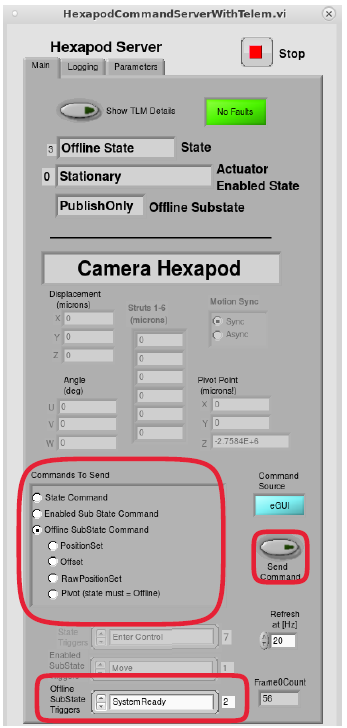
\includegraphics[width=1.79167in]{jira_imgs/1024.png}

}
\hdashrule[0.5ex]{\textwidth}{1pt}{3mm}
  Expected Result \\
{\footnotesize
The system transitions from the OfflineState/PublishOnly substate to the
OfflineState/AvailableState substate and the Command Source says
eGUI.\\[2\baselineskip]

}
\hdashrule[0.5ex]{\textwidth}{1pt}{3mm}
  Actual Result \\
{\footnotesize

}
\begin{tabular}{p{2cm}p{14cm}}
\toprule
Step 4 & Step Execution Status: \textbf{ Initial Pass } \\ \hline
\end{tabular}
 Description \\
{\footnotesize
\textbf{OFFLINESTATE -\textgreater{} STANDBYSTATE}\\
Click on the State Command field in the Commands to Send section.\\
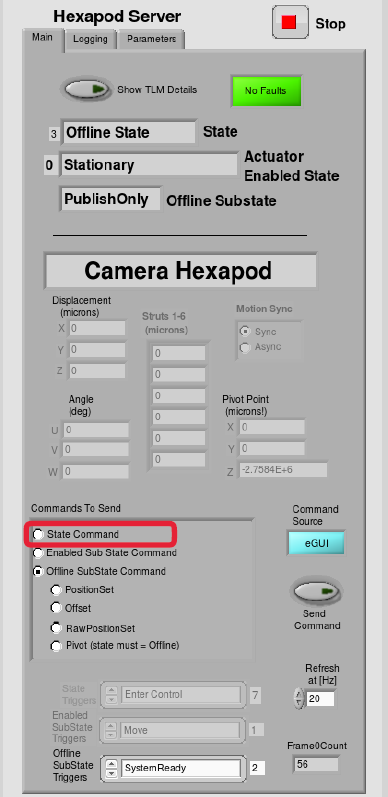
\includegraphics[width=1.79167in]{jira_imgs/1028.png}

}
\hdashrule[0.5ex]{\textwidth}{1pt}{3mm}
  Expected Result \\
{\footnotesize
The State Triggers dialogue box shown below becomes visible.\\
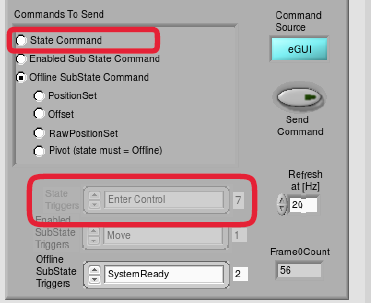
\includegraphics[width=1.79167in]{jira_imgs/1029.png}

}
\hdashrule[0.5ex]{\textwidth}{1pt}{3mm}
  Actual Result \\
{\footnotesize

}
\begin{tabular}{p{2cm}p{14cm}}
\toprule
Step 5 & Step Execution Status: \textbf{ Initial Pass } \\ \hline
\end{tabular}
 Description \\
{\footnotesize
Scroll through the available trigger options to select ``Enter Control''
and click the Send Command button.

}
\hdashrule[0.5ex]{\textwidth}{1pt}{3mm}
  Expected Result \\
{\footnotesize
The system transitions to the Standby state and the primary state
display box at the top of the Main says Standby State.

}
\hdashrule[0.5ex]{\textwidth}{1pt}{3mm}
  Actual Result \\
{\footnotesize

}
\begin{tabular}{p{2cm}p{14cm}}
\toprule
Step 6 & Step Execution Status: \textbf{ Initial Pass } \\ \hline
\end{tabular}
 Description \\
{\footnotesize
\textbf{STANDBYSTATE -\textgreater{} DISABLEDSTATE}\\
From the StandbyState, send a Start State command.

}
\hdashrule[0.5ex]{\textwidth}{1pt}{3mm}
  Expected Result \\
{\footnotesize
The system transitions into DisabledState and the current configuration
parameters are maintained from the default parameters or from the
previous DDS start command.~

}
\hdashrule[0.5ex]{\textwidth}{1pt}{3mm}
  Actual Result \\
{\footnotesize

}
\begin{tabular}{p{2cm}p{14cm}}
\toprule
Step 7 & Step Execution Status: \textbf{ Initial Pass } \\ \hline
\end{tabular}
 Description \\
{\footnotesize
\textbf{DISABLEDSTATE -\textgreater{} ENABLEDSTATE}\\
From the DisabledState, send an Enable State Command.~

}
\hdashrule[0.5ex]{\textwidth}{1pt}{3mm}
  Expected Result \\
{\footnotesize
The system transitions into the EnabledState/Stationary substate, the
motor drives are enabled and and motion can be commanded.~

}
\hdashrule[0.5ex]{\textwidth}{1pt}{3mm}
  Actual Result \\
{\footnotesize

}
\begin{tabular}{p{2cm}p{14cm}}
\toprule
Step 8 & Step Execution Status: \textbf{ Initial Pass } \\ \hline
\end{tabular}
 Description \\
{\footnotesize
\textless{}conditional state\textgreater{}\\
\textbf{FAULTSTATE}\\
If a Fault occurs in any of the other states, the system will
automatically transition to the Fault State. While in the Fault state,
send a clearError.\\
Note: If the fault that occurs goes through the interlock system, reset
the safety relay switch and send a clearError command.

}
\hdashrule[0.5ex]{\textwidth}{1pt}{3mm}
  Expected Result \\
{\footnotesize
The system transitions back to the OfflineState/PublishOnly substate.
(Go back to Step 3)

}
\hdashrule[0.5ex]{\textwidth}{1pt}{3mm}
  Actual Result \\
{\footnotesize

}
\begin{tabular}{p{2cm}p{14cm}}
\toprule
Step 9 & Step Execution Status: \textbf{ Fail } \\ \hline
\end{tabular}
 Description \\
{\footnotesize
\textbf{Follow \emph{3.5.12 Positioning~}of the LSST Hexapods-Rotator
Acceptance Test Procedure, Sheet 57-58.}

}
\hdashrule[0.5ex]{\textwidth}{1pt}{3mm}
  Test Data \\
 {\footnotesize
\textbf{Deviation}: Test at a single elevation angle.

}
\hdashrule[0.5ex]{\textwidth}{1pt}{3mm}
  Expected Result \\
{\footnotesize
The position of the hexapod is able to reach the commanded positions
within the absolute accuracy specifications of 25um in Z, 125um in XY,
83x10-5deg in RXRY, and 750x10-5deg in RZ.

}
\hdashrule[0.5ex]{\textwidth}{1pt}{3mm}
  Actual Result \\
{\footnotesize
The errors in XY are considered via sqrt(Xerr**2+Yerr**2) and
individually for each measurement.\\
The results for the test steps 25, 26, 27, 28, 30, and 32 are out of
specs.\\
See results in M2 hexapod\_the test moves\_02-25
Feb2021\_Results\_updateRT27042021\_comment\_hd column AB and AC from
line 34 on.

}
\hdashrule[0.5ex]{\textwidth}{1pt}{3mm}
  Issues found executing this step:  \\
{\footnotesize
\begin{itemize}
\item \href{https://jira.lsstcorp.org/browse/LVV-19511}{LVV-19511}~~M2 Hexapod absolute XYZ value accuracy not reached

\end{itemize}
}
\begin{tabular}{p{2cm}p{14cm}}
\toprule
Step 10 & Step Execution Status: \textbf{ Pass } \\ \hline
\end{tabular}
 Description \\
{\footnotesize
\textbf{Follow \emph{3.5.15 Radial (X and Y) Translation Range~}of
the}~\textbf{LSST Hexapods-Rotator Acceptance Test Procedure, Sheet 59.}

}
\hdashrule[0.5ex]{\textwidth}{1pt}{3mm}
  Test Data \\
 {\footnotesize
\textbf{Deviation}: Test at a single elevation angle.~{Wait for 39s
between each movement.}

}
\hdashrule[0.5ex]{\textwidth}{1pt}{3mm}
  Expected Result \\
{\footnotesize
The hexapod is capable of moving to the positions in the XY plane listed
in the Acceptance Test Procedure.

}
\hdashrule[0.5ex]{\textwidth}{1pt}{3mm}
  Actual Result \\
{\footnotesize
\textbf{Deviation:} In this test, the X and Y moves are up to a maximum
of 10mm not 10.05mm.\\
Hexapod reached the positions within the allowed tolerances and.\\
See lines 13-19, M2 hexapod\_the test moves\_02-25
Feb2021\_Results\_updateRT27042021\_comment\_hd

}
\begin{tabular}{p{2cm}p{14cm}}
\toprule
Step 11 & Step Execution Status: \textbf{ Initial Pass } \\ \hline
\end{tabular}
 Description \\
{\footnotesize
\textbf{Follow \emph{3.5.13 Centers of Rotation~}of the LSST
Hexapods-Rotator Acceptance Test Procedure, Sheet 58-59.}

}
\hdashrule[0.5ex]{\textwidth}{1pt}{3mm}
  Test Data \\
 {\footnotesize
\textbf{Deviation}: Test at a single elevation angle. Wait for 39s
between each movement. The spherically mounted retroreflector (SMR) will
be mounted on the ring holding the M2 mass surrogate or the M2 mass
simulator

}
\hdashrule[0.5ex]{\textwidth}{1pt}{3mm}
  Expected Result \\
{\footnotesize
The center of rotation is able to be moved.

}
\hdashrule[0.5ex]{\textwidth}{1pt}{3mm}
  Actual Result \\
{\footnotesize
initial pass. Details see page 6, M2 Hexapod
verification-tests\_2021.check\\
This was with the hexapod on level 3 in the ``zenith'' position. Test
again with hexapod at 0 elevations.

}
\begin{tabular}{p{2cm}p{14cm}}
\toprule
Step 12 & Step Execution Status: \textbf{ Initial Pass } \\ \hline
\end{tabular}
 Description \\
{\footnotesize
\textbf{Follow \emph{3.5.17 Axial (Z) Translation Range~}of the}
\textbf{LSST Hexapods-Rotator Acceptance Test Procedure, Sheet 60.}

}
\hdashrule[0.5ex]{\textwidth}{1pt}{3mm}
  Test Data \\
 {\footnotesize
\textbf{Deviation}: Test at a single elevation angle. {Wait for 39s
between each movement.}

}
\hdashrule[0.5ex]{\textwidth}{1pt}{3mm}
  Expected Result \\
{\footnotesize
The hexapod is capable of moving to the positions in the Z plane listed
in the Acceptance Test Procedure.

}
\hdashrule[0.5ex]{\textwidth}{1pt}{3mm}
  Actual Result \\
{\footnotesize
Initial pass. Hexapod moved to Z=8.9mm within the allowed tolerances.
See page 5, M2 Hexapod verification-tests\_2021.check4.

}
\begin{tabular}{p{2cm}p{14cm}}
\toprule
Step 13 & Step Execution Status: \textbf{ Initial Pass } \\ \hline
\end{tabular}
 Description \\
{\footnotesize
\textbf{Follow \emph{3.5.19 Rotational Range Around X-Axis (Tip) and
Y-Axis (Tilt)~}of the} \textbf{LSST Hexapods-Rotator Acceptance Test
Procedure, Sheet 61.}

}
\hdashrule[0.5ex]{\textwidth}{1pt}{3mm}
  Test Data \\
 {\footnotesize
\textbf{Deviation}: Test at a single elevation angle{. Wait for 39s
between each movement.}

}
\hdashrule[0.5ex]{\textwidth}{1pt}{3mm}
  Expected Result \\
{\footnotesize
The hexapod is capable of moving to the positions in the RXRY plane
listed in the Acceptance Test Procedure.

}
\hdashrule[0.5ex]{\textwidth}{1pt}{3mm}
  Actual Result \\
{\footnotesize
Initial pass. Hexapod moved to RX, RY = 0.175deg within the allowed
tolerances. See page 5, M2 Hexapod verification-tests\_2021.check4.

}
\begin{tabular}{p{2cm}p{14cm}}
\toprule
Step 14 & Step Execution Status: \textbf{ Initial Pass } \\ \hline
\end{tabular}
 Description \\
{\footnotesize
\textbf{Follow \emph{3.5.21 Rotation Range Around Z-Axis (Twist)~}of
the} \textbf{LSST Hexapods-Rotator Acceptance Test Procedure, Sheet 62.}

}
\hdashrule[0.5ex]{\textwidth}{1pt}{3mm}
  Test Data \\
 {\footnotesize
\textbf{Deviation}: Test at a single elevation angle. Wait for 39s
between each movement.

}
\hdashrule[0.5ex]{\textwidth}{1pt}{3mm}
  Expected Result \\
{\footnotesize
The hexapod is capable of moving to the positions in the RZ-axis listed
in the Acceptance Test Procedure.

}
\hdashrule[0.5ex]{\textwidth}{1pt}{3mm}
  Actual Result \\
{\footnotesize
Initial pass. Hexapod moved to the expected position within the allowed
tolerances. See page 5, M2 Hexapod verification-tests\_2021.check4.

}
\begin{tabular}{p{2cm}p{14cm}}
\toprule
Step 15 & Step Execution Status: \textbf{ Not Executed } \\ \hline
\end{tabular}
 Description \\
{\footnotesize
\textbf{Follow \emph{3.5.23 Hexapod Repeatability~}of the} \textbf{LSST
Hexapods-Rotator Acceptance Test Procedure, Sheet 63-70.}

}
\hdashrule[0.5ex]{\textwidth}{1pt}{3mm}
  Test Data \\
 {\footnotesize
\textbf{Deviation}: Allow a minimum of 30 seconds between moves.

}
\hdashrule[0.5ex]{\textwidth}{1pt}{3mm}
  Expected Result \\
{\footnotesize
The repeatability of the hexapod is likely better than can be determined
by the test equipment. This test will likely falsely show a deficiency
in the hexapod performance as a result of test equipment accuracy/
repeatability limitation.

}
\hdashrule[0.5ex]{\textwidth}{1pt}{3mm}
  Actual Result \\
{\footnotesize
See page 7, M2 Hexapod verification-tests\_2021.check4:~ Hexapod
repeatability tests\ldots{}not done, no time~

}
\begin{tabular}{p{2cm}p{14cm}}
\toprule
Step 16 & Step Execution Status: \textbf{ Fail } \\ \hline
\end{tabular}
 Description \\
{\footnotesize
\textbf{Follow \emph{3.5.24 Hexapod Absolute Accuracy~}of the}
\textbf{LSST Hexapods-Rotator Acceptance Test Procedure, Sheet 70-74.}

}
\hdashrule[0.5ex]{\textwidth}{1pt}{3mm}
  Test Data \\
 {\footnotesize
\textbf{Deviation}: Test at a single elevation angle.

}
\hdashrule[0.5ex]{\textwidth}{1pt}{3mm}
  Expected Result \\
{\footnotesize
The accuracy of the hexapod is at least the following:\\[2\baselineskip]

\begin{longtable}[]{@{}ll@{}}
\toprule
Axis & Required Accuracy (um, deg)\tabularnewline
\midrule
\endhead
X & 125\tabularnewline
Y & 125\tabularnewline
Z & 25\tabularnewline
RX & 0.00083\tabularnewline
RY & 0.00083\tabularnewline
RZ & 0.0075\tabularnewline
\bottomrule
\end{longtable}

\textbf{NOTE:~}The accuracy of the hexapod may be better than can be
determined by the test equipment. This may falsely show a deficiency in
the hexapod performance as a result of test equipment accuracy/
repeatability limitation.~

}
\hdashrule[0.5ex]{\textwidth}{1pt}{3mm}
  Actual Result \\
{\footnotesize
\textbf{Deviation:~}Only Z was tested.\\
Test failed the required accuracy. See page 8, M2 Hexapod
verification-tests\_2021.check4.\\
See lines 140-150, M2 hexapod\_the test moves\_02-25
Feb2021\_Results\_updateRT27042021\_comment\_hd

}
\hdashrule[0.5ex]{\textwidth}{1pt}{3mm}
  Issues found executing this step:  \\
{\footnotesize
\begin{itemize}
\item \href{https://jira.lsstcorp.org/browse/LVV-19511}{LVV-19511}~~M2 Hexapod absolute XYZ value accuracy not reached

\end{itemize}
}
\begin{tabular}{p{2cm}p{14cm}}
\toprule
Step 17 & Step Execution Status: \textbf{ Not Executed } \\ \hline
\end{tabular}
 Description \\
{\footnotesize
\textbf{Follow \emph{3.5.26 Hexapod Radial (X and Y) and Axial (Z)
Velocity Range}\textbf{~and \emph{3.5.27}}\emph{~Hexapod Rotational
Velocity~}of the} \textbf{LSST Hexapods-Rotator Acceptance Test
Procedure, Sheet 75.}

}
\hdashrule[0.5ex]{\textwidth}{1pt}{3mm}
  Test Data \\
 {\footnotesize
\textbf{Deviation:~}Only test this using synchronous mode. Wait for 39s
between each movement.

}
\hdashrule[0.5ex]{\textwidth}{1pt}{3mm}
  Expected Result \\
{\footnotesize
The hexapod velocity exceeds the 106um/s in XY and 0.0062deg/s in RXYRY
and RZ requirements.

}
\hdashrule[0.5ex]{\textwidth}{1pt}{3mm}
  Actual Result \\
{\footnotesize
Not tested

}
\begin{tabular}{p{2cm}p{14cm}}
\toprule
Step 18 & Step Execution Status: \textbf{ Not Executed } \\ \hline
\end{tabular}
 Description \\
{\footnotesize
\textbf{Follow 3.5.28\emph{~Hexapod Heat Dissipation} of the}
\textbf{LSST Hexapods-Rotator Acceptance Test Procedure, Sheet 75-76.}

}
\hdashrule[0.5ex]{\textwidth}{1pt}{3mm}
  Test Data \\
 {\footnotesize
\textbf{Deviation:~}Calculate the power by having an amp meter on the
legs. This test can be done simultaneously with the other test
steps.\\[2\baselineskip]

}
\hdashrule[0.5ex]{\textwidth}{1pt}{3mm}
  Expected Result \\
{\footnotesize
The current measured by the inductive current probes is calculated to
meet the heat dissipation requirement.

}
\hdashrule[0.5ex]{\textwidth}{1pt}{3mm}
  Actual Result \\
{\footnotesize
Not measured.

}
\begin{tabular}{p{2cm}p{14cm}}
\toprule
Step 19 & Step Execution Status: \textbf{ Not Executed } \\ \hline
\end{tabular}
 Description \\
{\footnotesize
\textbf{Follow \emph{3.5.14 Cross Talk Motion~}of the} \textbf{LSST
Hexapods-Rotator Acceptance Test Procedure, Sheet 59.}

}
\hdashrule[0.5ex]{\textwidth}{1pt}{3mm}
  Test Data \\
 {\footnotesize
\textbf{Deviation}: Analyze data from 3.5.15, 3.5.17, and 3.5.19 test
steps after testing to verify cross talk.~

}
\hdashrule[0.5ex]{\textwidth}{1pt}{3mm}
  Expected Result \\
{\footnotesize
There is no cross-talk observed.~

}
\hdashrule[0.5ex]{\textwidth}{1pt}{3mm}
  Actual Result \\
{\footnotesize

}

\paragraph{ LVV-T1802 - Integration of M2 Hexapod with SAL }\mbox{}\\

Version \textbf{2}.
Open  \href{https://jira.lsstcorp.org/secure/Tests.jspa#/testCase/LVV-T1802}{\textit{ LVV-T1802 } }
test case in Jira.

The objective of this test case is to re-verify the functional
requirements of the M2 hexapod's software, after shipment of the
hardware from the vendor's facility to the Summit, as defined in \citeds{LTS-206}
and \citeds{LTS-160}. This test case will only exercise the functionality that
was executed previously and meets the following criteria:

\begin{itemize}
\tightlist
\item
  Only requires the use of Rubin Observatory code to replace MOOG's
  middleware code
\item
  Only requires the M2 hexapod to be operable
\item
  Only requires command through the CSC after the PXI real-time
  controller is switched from GUI mode to DDS mode
\item
  Only requires testing the synchronous mode

  \begin{itemize}
  \tightlist
  \item
    \textbf{Asynchronous mode is not a standard mode of operation}
  \end{itemize}
\item
  Does require the M2 hexapod temperature sensors to be operating
\item
  Does \textbf{NOT} require the M2 hexapod to be rotated to various
  elevation angles.
\item
  Does \textbf{NOT~}require the M2 hexapod to be in a climate-controlled
  environment
\end{itemize}

The software functional requirements were previously verified during the
test campaign by the vendor at the vendor's facility and accepted by
Rubin Observatory during the Factory Acceptance Test review. The test
procedure used during the vendor's acceptance testing is the \emph{LSST
Hexapods-Rotator Software Acceptance Test Procedure} which is attached
to this test case. The test steps of this test case are the same steps
from the procedure for the testing of the Camera Hexapod. The order of
the steps was changed to reflect the \emph{Proposal of Hexapod Test~on
the Dec. 2019~}Confluence page which can be found linked in the
Traceability tab.\\[2\baselineskip]See the attached \emph{LSST Hexapod
Operator's Manual} for more information on how to operate the hexapod.

\textbf{ Preconditions}:\\
Prior to the execution of this test case to re-verify the M2 Hexapod
hardware functional requirements, the following Summit tasks must be
completed:

\begin{itemize}
\tightlist
\item
  The measurement equipment has been set-up for testing

  \begin{itemize}
  \tightlist
  \item
    \url{https://jira.lsstcorp.org/browse/SUMMIT-1943}
  \end{itemize}
\end{itemize}

Execution status: {\bf Fail }

Final comment:\\

Issues found during the execution of LVV-T1802 test case:

\begin{itemize}
\item \href{https://jira.lsstcorp.org/browse/LVV-19512}{LVV-19512}~~M2 Hexapod SAL verification failures

\item \href{https://jira.lsstcorp.org/browse/LVV-19512}{LVV-19512}~~M2 Hexapod SAL verification failures

\item \href{https://jira.lsstcorp.org/browse/LVV-19512}{LVV-19512}~~M2 Hexapod SAL verification failures

\item \href{https://jira.lsstcorp.org/browse/LVV-19512}{LVV-19512}~~M2 Hexapod SAL verification failures

\end{itemize}

Detailed steps results:

\begin{tabular}{p{2cm}p{14cm}}
\toprule
Step 1 & Step Execution Status: \textbf{ Pass } \\ \hline
\end{tabular}
 Description \\
{\footnotesize
\textbf{STARTING THE EUI}\\[2\baselineskip]Double click the Hexapod GUI
Viewer desktop icon on the computer.

\begin{itemize}
\tightlist
\item
  This can be done on the Dell Management PC or another computer on the
  same network
\end{itemize}

}
\hdashrule[0.5ex]{\textwidth}{1pt}{3mm}
  Expected Result \\
{\footnotesize
A prompt to enter a password is shown.~

}
\hdashrule[0.5ex]{\textwidth}{1pt}{3mm}
  Actual Result \\
{\footnotesize
See: LVV-E1022

}
\begin{tabular}{p{2cm}p{14cm}}
\toprule
Step 2 & Step Execution Status: \textbf{ Pass } \\ \hline
\end{tabular}
 Description \\
{\footnotesize
Enter the password ``lsst-vnc''

\begin{itemize}
\tightlist
\item
  If the EUI isn't automatically up and running when the VNC opens,
  double click on the Hexapod-eGUI icon on the VNC viewer
\end{itemize}

}
\hdashrule[0.5ex]{\textwidth}{1pt}{3mm}
  Expected Result \\
{\footnotesize
The EUI is in the Offline State/PublishOnly substate and is able to
publish through SAL but cannot receive commands.

}
\hdashrule[0.5ex]{\textwidth}{1pt}{3mm}
  Actual Result \\
{\footnotesize
See: LVV-E1022

}
\begin{tabular}{p{2cm}p{14cm}}
\toprule
Step 3 & Step Execution Status: \textbf{ Initial Pass } \\ \hline
\end{tabular}
 Description \\
{\footnotesize
\textbf{OFFLINESTATE/PUBLISHONLY -\textgreater{}
OFFLINESTATE/AVAILABLESTATE}\\
On the Main tab, select the ``Offline SubState Cmd'' field in the
Commands to Send section, set the Offline SubState Triggers to ``System
Ready'' and click on the Send Command button.\\
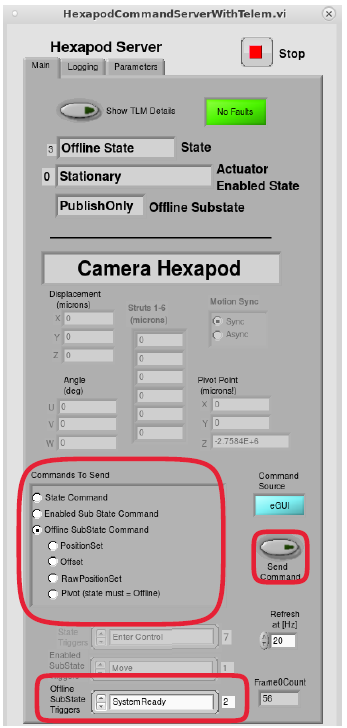
\includegraphics[width=1.79167in]{jira_imgs/1024.png}

}
\hdashrule[0.5ex]{\textwidth}{1pt}{3mm}
  Expected Result \\
{\footnotesize
The system transitions from the OfflineState/PublishOnly substate to the
OfflineState/AvailableState substate.\\[2\baselineskip]

}
\hdashrule[0.5ex]{\textwidth}{1pt}{3mm}
  Actual Result \\
{\footnotesize
See: LVV-E1022

}
\begin{tabular}{p{2cm}p{14cm}}
\toprule
Step 4 & Step Execution Status: \textbf{ Initial Pass } \\ \hline
\end{tabular}
 Description \\
{\footnotesize
\textbf{SWITCHING TO DDS MODE}\\
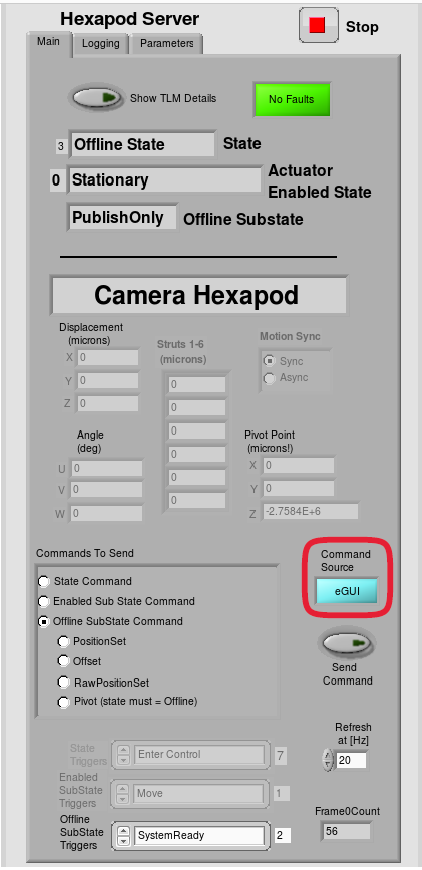
\includegraphics[width=1.68750in]{jira_imgs/1025.png}If the Command
Source does not show DDS, go to the Parameters tab, select DDS under the
Command Source and click the Set Cmd Source button.\\
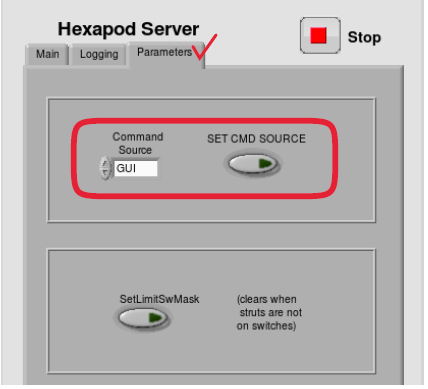
\includegraphics[width=2.34375in]{jira_imgs/1026.png}\textbf{Note:~If
the GUI is used after being set to DDS mode, the system will switch back
the Command Source to GUI and ignore any DDS commands. The Command
Source must show DDS in order to receive DDS commands.}

}
\hdashrule[0.5ex]{\textwidth}{1pt}{3mm}
  Expected Result \\
{\footnotesize
The system is capable of receiving/responding to DDS commands.

}
\hdashrule[0.5ex]{\textwidth}{1pt}{3mm}
  Actual Result \\
{\footnotesize
See: LVV-E1022

}
\begin{tabular}{p{2cm}p{14cm}}
\toprule
Step 5 & Step Execution Status: \textbf{ Initial Pass } \\ \hline
\end{tabular}
 Description \\
{\footnotesize
\textbf{OFFLINESTATE -\textgreater{} STANDBYSTATE}\\
The system receives an enterControl State Transition command through
DDS.

}
\hdashrule[0.5ex]{\textwidth}{1pt}{3mm}
  Expected Result \\
{\footnotesize
The system transitions into the StandbyState and is capable of
receiving/responding to DDS commands.

}
\hdashrule[0.5ex]{\textwidth}{1pt}{3mm}
  Actual Result \\
{\footnotesize
See: LVV-E1022

}
\begin{tabular}{p{2cm}p{14cm}}
\toprule
Step 6 & Step Execution Status: \textbf{ Initial Pass } \\ \hline
\end{tabular}
 Description \\
{\footnotesize
\textbf{STANDBYSTATE -\textgreater{} DISABLEDSTATE}\\
From the StandbyState, send a start command through the DDS.

}
\hdashrule[0.5ex]{\textwidth}{1pt}{3mm}
  Expected Result \\
{\footnotesize
The system transitions into DisabledState after receiving/responding to
DDS command and the wrapper in the PXI real time controller looks for
the configuration file.\\[2\baselineskip]If the configuration file is
invalid or out of range, the system will transition into a Fault State

}
\hdashrule[0.5ex]{\textwidth}{1pt}{3mm}
  Actual Result \\
{\footnotesize
See: LVV-E1022

}
\begin{tabular}{p{2cm}p{14cm}}
\toprule
Step 7 & Step Execution Status: \textbf{ Initial Pass } \\ \hline
\end{tabular}
 Description \\
{\footnotesize
\textbf{DISABLEDSTATE -\textgreater{} ENABLEDSTATE}\\
From the DisabledState, send an enable state command through the DDS.\\
\textbf{}

}
\hdashrule[0.5ex]{\textwidth}{1pt}{3mm}
  Expected Result \\
{\footnotesize
The system transitions into the EnabledState/Stationary substate, the
motor drives are enabled, motor brakes are released and the system is
capable of receiving/responding to DDS commands.\\[2\baselineskip]

}
\hdashrule[0.5ex]{\textwidth}{1pt}{3mm}
  Actual Result \\
{\footnotesize
See: LVV-E1022

}
\begin{tabular}{p{2cm}p{14cm}}
\toprule
Step 8 & Step Execution Status: \textbf{ Initial Pass } \\ \hline
\end{tabular}
 Description \\
{\footnotesize
\textbf{FAULTSTATE}\\
If a Fault occurs in any of the other states, the system will
automatically transition to the Fault State. While in the Fault state,
send a clearError command through the DDS.\\
Note: If the fault that occurs goes through the interlock system, reset
the safety relay switch and send a clearError command.

}
\hdashrule[0.5ex]{\textwidth}{1pt}{3mm}
  Expected Result \\
{\footnotesize
The system transitions back to the OfflineState/PublishOnly substate and
is not capable of receiving/responding to DDS commands. (Go back to Step
3)

}
\hdashrule[0.5ex]{\textwidth}{1pt}{3mm}
  Actual Result \\
{\footnotesize
See: LVV-E1022

}
\begin{tabular}{p{2cm}p{14cm}}
\toprule
Step 9 & Step Execution Status: \textbf{ Initial Pass } \\ \hline
\end{tabular}
 Description \\
{\footnotesize
Verify that the thermal sensors are connected and producing telemetry
into the EFD.\\[2\baselineskip]

}
\hdashrule[0.5ex]{\textwidth}{1pt}{3mm}
  Expected Result \\
{\footnotesize
All actuator temperatures are published to the EFD.

}
\hdashrule[0.5ex]{\textwidth}{1pt}{3mm}
  Actual Result \\
{\footnotesize
Deviation: Thermal sensors were not available during this test. Instead,
a waiting time of at least 39sec between each move was used to ensure
that the hexapod does not overheat.

}
\begin{tabular}{p{2cm}p{14cm}}
\toprule
Step 10 & Step Execution Status: \textbf{ Initial Pass } \\ \hline
\end{tabular}
 Description \\
{\footnotesize
The following steps define what the Jupyter Notebook for this test case
implements. Executing the Jupyter notebook is the only actual command
and control step that needs to be executed.

}
\hdashrule[0.5ex]{\textwidth}{1pt}{3mm}
  Expected Result \\
{\footnotesize
The Jupyter notebook controls the system to run through the steps below.

}
\hdashrule[0.5ex]{\textwidth}{1pt}{3mm}
  Actual Result \\
{\footnotesize
Yes, a Jupiter notebook can be used to control the hexapod. Notebook is
named lvv-t1802.ipynb

}
\begin{tabular}{p{2cm}p{14cm}}
\toprule
Step 11 & Step Execution Status: \textbf{ Initial Pass } \\ \hline
\end{tabular}
 Description \\
{\footnotesize
Verify all the telemetry is being ingested into the EFD.

}
\hdashrule[0.5ex]{\textwidth}{1pt}{3mm}
  Expected Result \\
{\footnotesize
All telemetry defined in the script is being ingested into the EFD.

}
\hdashrule[0.5ex]{\textwidth}{1pt}{3mm}
  Actual Result \\
{\footnotesize
\textbf{Deviation:}\\

\begin{itemize}
\tightlist
\item
  CSC and KAFKA producer needed to be restarted
\end{itemize}

}
\begin{tabular}{p{2cm}p{14cm}}
\toprule
Step 12 & Step Execution Status: \textbf{ Pass } \\ \hline
\end{tabular}
 Description \\
{\footnotesize
\textbf{{MOVE TEST}}\\
\textbf{Section 3.1.2 of the attached Software Acceptance Test
Procedure\\
Test Sequence \#1 - Synchronous PositionSet and Move Commands}\\
In enabled/stationary state, send a positionSet command of (0um, 0um,
200um, 0 deg, 0 deg, 0 deg, s).

}
\hdashrule[0.5ex]{\textwidth}{1pt}{3mm}
  Test Data \\
 {\footnotesize
\textbf{Deviation:~}Skip this step. positionSet and move command
replaced by new move command. Now, the hexapod starts movement directly
after receiving the command.

}
\hdashrule[0.5ex]{\textwidth}{1pt}{3mm}
  Expected Result \\
{\footnotesize
The hexapod does not move.

}
\hdashrule[0.5ex]{\textwidth}{1pt}{3mm}
  Actual Result \\
{\footnotesize

}
\begin{tabular}{p{2cm}p{14cm}}
\toprule
Step 13 & Step Execution Status: \textbf{ Pass } \\ \hline
\end{tabular}
 Description \\
{\footnotesize
With the synchronous button enabled and in enabled/stationary state,
send a positionSet command of (500um, -500um, 200um, 0.01deg, -0.015deg,
0deg).

}
\hdashrule[0.5ex]{\textwidth}{1pt}{3mm}
  Test Data \\
 {\footnotesize
\textbf{Deviation:~}Skip this step. positionSet and move command
replaced by new move command. Now, the hexapod starts movement directly
after receiving the command.

}
\hdashrule[0.5ex]{\textwidth}{1pt}{3mm}
  Expected Result \\
{\footnotesize
The hexapod does not move

}
\hdashrule[0.5ex]{\textwidth}{1pt}{3mm}
  Actual Result \\
{\footnotesize

}
\begin{tabular}{p{2cm}p{14cm}}
\toprule
Step 14 & Step Execution Status: \textbf{ Initial Pass } \\ \hline
\end{tabular}
 Description \\
{\footnotesize
With the hexapod in in enabled/stationary state sync=True and send the
move command of (x= 500um,y= -500um, z=200um, u=0.01deg, v=-0.015deg,
w=0deg).

}
\hdashrule[0.5ex]{\textwidth}{1pt}{3mm}
  Expected Result \\
{\footnotesize
\begin{itemize}
\tightlist
\item
  The hexapod moves to (x= 500um,y= -500um, z=200um, u=0.01deg,
  v=-0.015deg, w=0deg)
\item
  Since the Hexapod is in synchronous mode, the actuators complete the
  move at nearly the same time.
\end{itemize}

}
\hdashrule[0.5ex]{\textwidth}{1pt}{3mm}
  Actual Result \\
{\footnotesize
The M2 hexapod moved as expected to the commanded position
(x=500,y=-500,z=200, u=0.01,v=-0.015,w=0,sync=True) all actuators
reached the position nearly at the same time.\\[2\baselineskip]Results
from the EFD from before and after the movement:\\[2\baselineskip]hex
position\\
0.05 0.30 -0.36 -0.00 0.00 0.00\\[2\baselineskip]hex position\\
500.24 -500.36 199.90 0.01 -0.02 0.00

}
\begin{tabular}{p{2cm}p{14cm}}
\toprule
Step 15 & Step Execution Status: \textbf{ Fail } \\ \hline
\end{tabular}
 Description \\
{\footnotesize
Record the corresponding DDS events that were generated.

}
\hdashrule[0.5ex]{\textwidth}{1pt}{3mm}
  Expected Result \\
{\footnotesize
\begin{itemize}
\tightlist
\item
  The controllerState.enabledSubstate goes to MOVING\_POINT\_TO\_POINT
  when the move begins and STATIONARY when the move ends.
\item
  An inPosition event is generated when the move is complete
\end{itemize}

}
\hdashrule[0.5ex]{\textwidth}{1pt}{3mm}
  Actual Result \\
{\footnotesize
\begin{itemize}
\tightlist
\item
  Expected results from the EFD:

  \begin{enumerate}
  \tightlist
  \item
    EnabledSubstate.MOVING\_POINT\_TO\_POINT
  \item
    EnabledSubstate.STATIONARY
  \end{enumerate}
\item
  {Fail:~}The \emph{inPosition} events were not generated.
\end{itemize}

}
\hdashrule[0.5ex]{\textwidth}{1pt}{3mm}
  Issues found executing this step:  \\
{\footnotesize
\begin{itemize}
\item \href{https://jira.lsstcorp.org/browse/LVV-19512}{LVV-19512}~~M2 Hexapod SAL verification failures

\end{itemize}
}
\begin{tabular}{p{2cm}p{14cm}}
\toprule
Step 16 & Step Execution Status: \textbf{ Pass } \\ \hline
\end{tabular}
 Description \\
{\footnotesize
Wait 39 seconds.\\[2\baselineskip]

}
\hdashrule[0.5ex]{\textwidth}{1pt}{3mm}
  Expected Result \\
{\footnotesize

}
\hdashrule[0.5ex]{\textwidth}{1pt}{3mm}
  Actual Result \\
{\footnotesize

}
\begin{tabular}{p{2cm}p{14cm}}
\toprule
Step 17 & Step Execution Status: \textbf{ Initial Pass } \\ \hline
\end{tabular}
 Description \\
{\footnotesize
Record the corresponding thermal sensors and verify they are below 19
deg C. If they are above 19 deg C, wait until they are below 19 deg C to
perform the following steps.

}
\hdashrule[0.5ex]{\textwidth}{1pt}{3mm}
  Expected Result \\
{\footnotesize
All actuators are below 19 deg C.\\[2\baselineskip]

}
\hdashrule[0.5ex]{\textwidth}{1pt}{3mm}
  Actual Result \\
{\footnotesize
Sensors not available.

}
\begin{tabular}{p{2cm}p{14cm}}
\toprule
Step 18 & Step Execution Status: \textbf{ Initial Pass } \\ \hline
\end{tabular}
 Description \\
{\footnotesize
\textbf{Section 3.1.2 of the attached Software Acceptance Test
Procedure\\
Test Sequence \#5 - Stop Commands}\\
In the enabled/stationary state, send a move command of (x=0um, y=0um,
z=5000um, u=0deg, v=0deg, w=0deg)

}
\hdashrule[0.5ex]{\textwidth}{1pt}{3mm}
  Expected Result \\
{\footnotesize
The hexapod doesn't move.

}
\hdashrule[0.5ex]{\textwidth}{1pt}{3mm}
  Actual Result \\
{\footnotesize
Hexapod started to move.\\[2\baselineskip]

}
\begin{tabular}{p{2cm}p{14cm}}
\toprule
Step 19 & Step Execution Status: \textbf{ Initial Pass } \\ \hline
\end{tabular}
 Description \\
{\footnotesize
Wait 3s.

}
\hdashrule[0.5ex]{\textwidth}{1pt}{3mm}
  Expected Result \\
{\footnotesize

}
\hdashrule[0.5ex]{\textwidth}{1pt}{3mm}
  Actual Result \\
{\footnotesize
This is a wait statement in the code.\\[2\baselineskip]

}
\begin{tabular}{p{2cm}p{14cm}}
\toprule
Step 20 & Step Execution Status: \textbf{ Initial Pass } \\ \hline
\end{tabular}
 Description \\
{\footnotesize
Send a stop command.

}
\hdashrule[0.5ex]{\textwidth}{1pt}{3mm}
  Expected Result \\
{\footnotesize
\begin{itemize}
\tightlist
\item
  The hexapod stops before reaching the previously commanded position
\end{itemize}

}
\hdashrule[0.5ex]{\textwidth}{1pt}{3mm}
  Actual Result \\
{\footnotesize
Hexapod stopped

}
\begin{tabular}{p{2cm}p{14cm}}
\toprule
Step 21 & Step Execution Status: \textbf{ Fail } \\ \hline
\end{tabular}
 Description \\
{\footnotesize
Record the corresponding DDS events that were generated.

}
\hdashrule[0.5ex]{\textwidth}{1pt}{3mm}
  Expected Result \\
{\footnotesize
\begin{itemize}
\tightlist
\item
  The controllerState.enabledSubstate goes to CONTROLLED\_STOPPING when
  the stop is requested, then STATIONARY when the hexapod has halted.
\item
  No inPosition event is generated.
\end{itemize}

}
\hdashrule[0.5ex]{\textwidth}{1pt}{3mm}
  Actual Result \\
{\footnotesize
The hexapod moved and stop before finishing the movement.

~

{FAIL:}~ controllerState.enabledSubstate goes to CONTROLLED\_STOPPING :
CONTROLLED\_STOPPING not reported.

~

~

Results from the EFD from before and after the movement:

~

\begin{verbatim}
INFO:Script:START- M2 Hexapod Integration Test -- LVV-T1802 Test Step 11
\end{verbatim}

\begin{verbatim}
 
\end{verbatim}

\begin{verbatim}
hex position
\end{verbatim}

\begin{verbatim}
      0.16        0.45       -0.34       -0.00        0.00        0.00  
\end{verbatim}

\begin{verbatim}
 
\end{verbatim}

\begin{verbatim}
EnabledSubstate.MOVING_POINT_TO_POINT
\end{verbatim}

\begin{verbatim}
EnabledSubstate.STATIONARY
\end{verbatim}

\begin{verbatim}
 
\end{verbatim}

\begin{verbatim}
INFO:Script:STOP- M2 Hexapod Integration Test -- LVV-T1802 Test Step 11
\end{verbatim}

\begin{verbatim}
 
\end{verbatim}

\begin{verbatim}
hex position
\end{verbatim}

\begin{verbatim}
     -9.43       17.09     1241.17        0.00       -0.00        0.00 
\end{verbatim}

~

}
\hdashrule[0.5ex]{\textwidth}{1pt}{3mm}
  Issues found executing this step:  \\
{\footnotesize
\begin{itemize}
\item \href{https://jira.lsstcorp.org/browse/LVV-19512}{LVV-19512}~~M2 Hexapod SAL verification failures

\end{itemize}
}
\begin{tabular}{p{2cm}p{14cm}}
\toprule
Step 22 & Step Execution Status: \textbf{ Pass } \\ \hline
\end{tabular}
 Description \\
{\footnotesize
Wait 39 seconds.

}
\hdashrule[0.5ex]{\textwidth}{1pt}{3mm}
  Expected Result \\
{\footnotesize

}
\hdashrule[0.5ex]{\textwidth}{1pt}{3mm}
  Actual Result \\
{\footnotesize

}
\begin{tabular}{p{2cm}p{14cm}}
\toprule
Step 23 & Step Execution Status: \textbf{ Initial Pass } \\ \hline
\end{tabular}
 Description \\
{\footnotesize
Record the corresponding thermal sensors and verify they are below 19
deg C. If they are above 19 deg C, wait until they are below 19 deg C to
perform the following steps.

}
\hdashrule[0.5ex]{\textwidth}{1pt}{3mm}
  Expected Result \\
{\footnotesize
All actuators are below 19 deg C.

}
\hdashrule[0.5ex]{\textwidth}{1pt}{3mm}
  Actual Result \\
{\footnotesize
see above.

}
\begin{tabular}{p{2cm}p{14cm}}
\toprule
Step 24 & Step Execution Status: \textbf{ Initial Pass } \\ \hline
\end{tabular}
 Description \\
{\footnotesize
\textbf{Section 3.1.2 of the attached Software Acceptance Test
Procedure\\
Test Sequence \#9 - positionSet and
moveLUT}\\[2\baselineskip]\textbf{Update: Test the
``setCompensationMode'' command.}\\[2\baselineskip]In enabled/stationary
state, send a move command of (x=0um, y=0um, z=800um, u=0deg, v=0deg,
w=0deg)\\[4\baselineskip]

}
\hdashrule[0.5ex]{\textwidth}{1pt}{3mm}
  Test Data \\
 {\footnotesize
\textbf{Deviation:} There is no ``positionSet'' and no ``moveLUT''
command anymore. ``positionSet'' and ``move'' command replaced by new
``move'' command. Now, the hexapod starts movement directly after
receiving the command. moveLUT is replaced by a ``setCompensationMode''.

}
\hdashrule[0.5ex]{\textwidth}{1pt}{3mm}
  Expected Result \\
{\footnotesize
The hexapod moves to the position (x=0um, y=0um, z=800um, u=0deg,
v=0deg, w=0deg) and, since we are moving in synchronous mode, the
actuators complete the move at nearly the same time.

}
\hdashrule[0.5ex]{\textwidth}{1pt}{3mm}
  Actual Result \\
{\footnotesize
Hexapod moved back to (x=0,y=0,z=0, u=0,v=0,w=0,sync=True).

Wait 39sec.

~

Move to (x=0um, y=0um, z=800um, u=0deg, v=0deg, w=0deg) worked.

~

Results from the EFD from after the movement:

\begin{verbatim}
INFO:Script:START- M2 Hexapod Integration Test -- LVV-T1802 Test Step 17
\end{verbatim}

\begin{verbatim}
 
\end{verbatim}

\begin{verbatim}
EnabledSubstate.MOVING_POINT_TO_POINT
\end{verbatim}

\begin{verbatim}
EnabledSubstate.STATIONARY
\end{verbatim}

\begin{verbatim}
 
\end{verbatim}

\begin{verbatim}
hex position
\end{verbatim}

\begin{verbatim}
     -0.09        0.00      799.94       -0.00       -0.00        0.00
\end{verbatim}

~

}
\begin{tabular}{p{2cm}p{14cm}}
\toprule
Step 25 & Step Execution Status: \textbf{ Initial Pass } \\ \hline
\end{tabular}
 Description \\
{\footnotesize
Ensure that MTMount publishes the telescope elevation angle and
MTRotator publishes the rotation angle of the rotator. Either as real
components or through controllers simulating the components.

}
\hdashrule[0.5ex]{\textwidth}{1pt}{3mm}
  Expected Result \\
{\footnotesize
Published telescope elevation and rotator angle.

}
\hdashrule[0.5ex]{\textwidth}{1pt}{3mm}
  Actual Result \\
{\footnotesize

}
\begin{tabular}{p{2cm}p{14cm}}
\toprule
Step 26 & Step Execution Status: \textbf{ Initial Pass } \\ \hline
\end{tabular}
 Description \\
{\footnotesize
In enabled/stationary state, set ~``setCompensationMode'' command to
enable=True.

}
\hdashrule[0.5ex]{\textwidth}{1pt}{3mm}
  Expected Result \\
{\footnotesize
The hexapod does not move and the MTHexapod.command\_setCompensationMode
appears as true in the
EFD.\\[2\baselineskip]logevent\_compensatedPosition is sent to the
EFD.\\[2\baselineskip]

}
\hdashrule[0.5ex]{\textwidth}{1pt}{3mm}
  Actual Result \\
{\footnotesize
Compensation mode switched activated on demand.

~

Results from the EFD from after the movement:

~

\begin{verbatim}
compsensation mode enabled? True
\end{verbatim}

\begin{verbatim}
hex position
\end{verbatim}

\begin{verbatim}
     -0.09        0.00      799.94       -0.00       -0.00        0.00  
\end{verbatim}

\begin{verbatim}
 
\end{verbatim}

\begin{verbatim}
EnabledSubstate.MOVING_POINT_TO_POINT
\end{verbatim}

\begin{verbatim}
EnabledSubstate.STATIONARY
\end{verbatim}

\begin{verbatim}
EnabledSubstate.MOVING_POINT_TO_POINT
\end{verbatim}

\begin{verbatim}
EnabledSubstate.STATIONARY
\end{verbatim}

\begin{verbatim}
EnabledSubstate.MOVING_POINT_TO_POINT
\end{verbatim}

\begin{verbatim}
EnabledSubstate.STATIONARY
\end{verbatim}

\begin{verbatim}
EnabledSubstate.MOVING_POINT_TO_POINT
\end{verbatim}

\begin{verbatim}
EnabledSubstate.STATIONARY
\end{verbatim}

\begin{verbatim}
EnabledSubstate.MOVING_POINT_TO_POINT
\end{verbatim}

\begin{verbatim}
EnabledSubstate.STATIONARY
\end{verbatim}

\begin{verbatim}
EnabledSubstate.MOVING_POINT_TO_POINT
\end{verbatim}

\begin{verbatim}
EnabledSubstate.STATIONARY
\end{verbatim}

\begin{verbatim}
EnabledSubstate.MOVING_POINT_TO_POINT
\end{verbatim}

\begin{verbatim}
EnabledSubstate.STATIONARY
\end{verbatim}

\begin{verbatim}
EnabledSubstate.MOVING_POINT_TO_POINT
\end{verbatim}

\begin{verbatim}
EnabledSubstate.STATIONARY
\end{verbatim}

\begin{verbatim}
EnabledSubstate.MOVING_POINT_TO_POINT
\end{verbatim}

\begin{verbatim}
EnabledSubstate.STATIONARY
\end{verbatim}

\begin{verbatim}
EnabledSubstate.MOVING_POINT_TO_POINT
\end{verbatim}

\begin{verbatim}
EnabledSubstate.STATIONARY
\end{verbatim}

\begin{verbatim}
EnabledSubstate.MOVING_POINT_TO_POINT
\end{verbatim}

\begin{verbatim}
EnabledSubstate.STATIONARY
\end{verbatim}

\begin{verbatim}
EnabledSubstate.MOVING_POINT_TO_POINT
\end{verbatim}

\begin{verbatim}
EnabledSubstate.STATIONARY
\end{verbatim}

\begin{verbatim}
EnabledSubstate.MOVING_POINT_TO_POINT
\end{verbatim}

}
\begin{tabular}{p{2cm}p{14cm}}
\toprule
Step 27 & Step Execution Status: \textbf{ Fail } \\ \hline
\end{tabular}
 Description \\
{\footnotesize
In enabled/stationary state, send a move command of (0um, 0um, 800um,
0deg, 0deg, 0deg)

}
\hdashrule[0.5ex]{\textwidth}{1pt}{3mm}
  Expected Result \\
{\footnotesize
The hexapod moves to a slightly different position than (0um, 0um,
800um, 0deg, 0deg, 0deg) and, since we are moving in synchronous mode,
the actuators complete the move at nearly the same time.

}
\hdashrule[0.5ex]{\textwidth}{1pt}{3mm}
  Actual Result \\
{\footnotesize
\begin{itemize}
\tightlist
\item
  {Fail:~}Sending a move command while in compensation mode it failed.
  Command arrives probably during: ~ ~
\end{itemize}

\begin{verbatim}
        EnabledSubstate.MOVING_POINT_TO_POINT
\end{verbatim}

In this substate, no move command can be received?

~

\begin{itemize}
\tightlist
\item
  Also, the code does not execute the next lines to stop the
  compensation mode. It can be stopped with a separately executed
  setCompensationMode=False command.
\end{itemize}

}
\hdashrule[0.5ex]{\textwidth}{1pt}{3mm}
  Issues found executing this step:  \\
{\footnotesize
\begin{itemize}
\item \href{https://jira.lsstcorp.org/browse/LVV-19512}{LVV-19512}~~M2 Hexapod SAL verification failures

\end{itemize}
}
\begin{tabular}{p{2cm}p{14cm}}
\toprule
Step 28 & Step Execution Status: \textbf{ Fail } \\ \hline
\end{tabular}
 Description \\
{\footnotesize
{Check if there are any different events between move with and without
setCompensationMode=True. Check the movement in the EFD use:\\
Compare logevent\_compensatedPosition to
logevent\_uncompensatedPosition}{\\
}

}
\hdashrule[0.5ex]{\textwidth}{1pt}{3mm}
  Expected Result \\
{\footnotesize
The changes are expected according to this table:\\
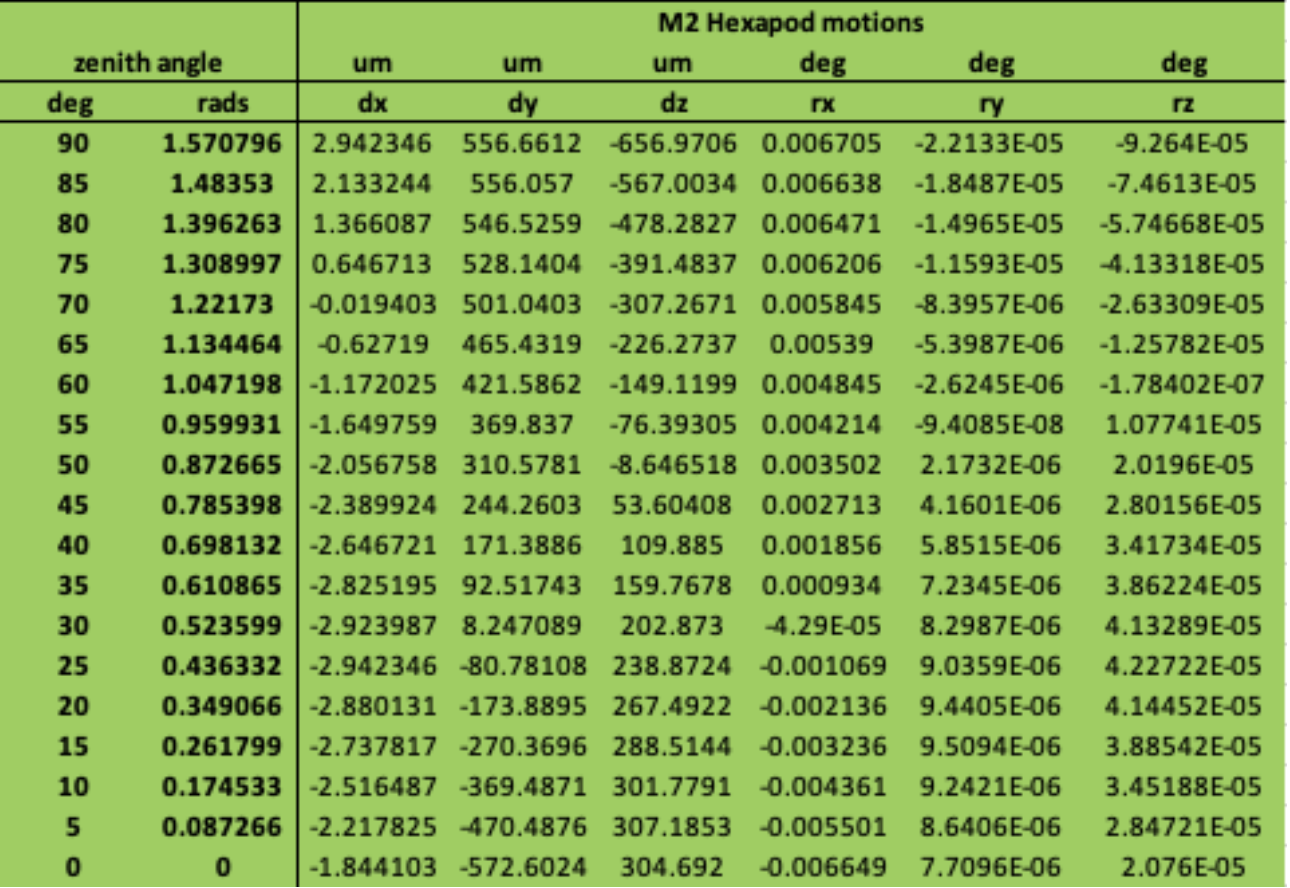
\includegraphics[width=3.12500in]{jira_imgs/1620.png}

}
\hdashrule[0.5ex]{\textwidth}{1pt}{3mm}
  Actual Result \\
{\footnotesize
\begin{itemize}
\tightlist
\item
  {{Fail???:}~}No compensation was applied. Results from EFD in the
  notebook and in Chronograph are the same. BUT this might be a
  consequence of a missing "\emph{inPosition"} event. See step 8.
\end{itemize}

~

\begin{itemize}
\tightlist
\item
  INFO:Script:START- M2 Hexapod Integration Test -- LVV-T1802 Test Step
  17
\item
  EnabledSubstate.MOVING\_POINT\_TO\_POINT
\item
  EnabledSubstate.STATIONARY
\item
  hex position
\item
  ~ ~ ~-0.09 ~ ~ ~ ~0.00 ~ ~ ~799.94 ~ ~ ~ -0.00 ~ ~ ~ -0.00 ~ ~ ~ ~0.00
  ~
\item
  ~
\item
  compsensation mode enabled? True
\item
  hex position
\item
  ~ ~ ~-0.09 ~ ~ ~ ~0.00 ~ ~ ~799.94 ~ ~ ~ -0.00 ~ ~ ~ -0.00 ~ ~ ~ ~0.00
  ~
\item
  ~
\item
  EnabledSubstate.MOVING\_POINT\_TO\_POINT
\item
  EnabledSubstate.STATIONARY
\item
  EnabledSubstate.MOVING\_POINT\_TO\_POINT
\item
  EnabledSubstate.STATIONARY
\item
  EnabledSubstate.MOVING\_POINT\_TO\_POINT
\item
  EnabledSubstate.STATIONARY
\item
  EnabledSubstate.MOVING\_POINT\_TO\_POINT
\item
  EnabledSubstate.STATIONARY
\item
  EnabledSubstate.MOVING\_POINT\_TO\_POINT
\item
  EnabledSubstate.STATIONARY
\item
  EnabledSubstate.MOVING\_POINT\_TO\_POINT
\item
  EnabledSubstate.STATIONARY
\item
  EnabledSubstate.MOVING\_POINT\_TO\_POINT
\item
  EnabledSubstate.STATIONARY
\item
  EnabledSubstate.MOVING\_POINT\_TO\_POINT
\item
  EnabledSubstate.STATIONARY
\item
  EnabledSubstate.MOVING\_POINT\_TO\_POINT
\item
  EnabledSubstate.STATIONARY
\item
  EnabledSubstate.MOVING\_POINT\_TO\_POINT
\item
  EnabledSubstate.STATIONARY
\item
  EnabledSubstate.MOVING\_POINT\_TO\_POINT
\item
  EnabledSubstate.STATIONARY
\item
  EnabledSubstate.MOVING\_POINT\_TO\_POINT
\item
  EnabledSubstate.STATIONARY
\item
  EnabledSubstate.MOVING\_POINT\_TO\_POINT
\item
  INFO:Script:STOP- M2 Hexapod Integration Test -- LVV-T1802 Test Step
  17
\item
  hex position
\item
  ~ ~ ~-0.09 ~ ~ ~ ~0.00 ~ ~ ~799.94 ~ ~ ~ -0.00 ~ ~ ~ -0.00 ~ ~ ~ ~0.00
\end{itemize}

~

}
\begin{tabular}{p{2cm}p{14cm}}
\toprule
Step 29 & Step Execution Status: \textbf{ Not Executed } \\ \hline
\end{tabular}
 Description \\
{\footnotesize
In enabled/stationary state, send again the same move command of (0um,
0um, 800um, 0deg, 0deg, 0deg)

}
\hdashrule[0.5ex]{\textwidth}{1pt}{3mm}
  Expected Result \\
{\footnotesize
The hexapod does not move since it stayed in compensationMode.

}
\hdashrule[0.5ex]{\textwidth}{1pt}{3mm}
  Actual Result \\
{\footnotesize
No tested

}
\begin{tabular}{p{2cm}p{14cm}}
\toprule
Step 30 & Step Execution Status: \textbf{ Pass } \\ \hline
\end{tabular}
 Description \\
{\footnotesize
Wait 39 seconds.

}
\hdashrule[0.5ex]{\textwidth}{1pt}{3mm}
  Expected Result \\
{\footnotesize

}
\hdashrule[0.5ex]{\textwidth}{1pt}{3mm}
  Actual Result \\
{\footnotesize

}
\begin{tabular}{p{2cm}p{14cm}}
\toprule
Step 31 & Step Execution Status: \textbf{ Initial Pass } \\ \hline
\end{tabular}
 Description \\
{\footnotesize
Record the corresponding thermal sensors and verify they are below 19
deg C. If they are above 19 deg C, wait until they are below 19 deg C to
perform the following steps.

}
\hdashrule[0.5ex]{\textwidth}{1pt}{3mm}
  Expected Result \\
{\footnotesize
All actuators are below 19 deg C.

}
\hdashrule[0.5ex]{\textwidth}{1pt}{3mm}
  Actual Result \\
{\footnotesize
see above

}
\begin{tabular}{p{2cm}p{14cm}}
\toprule
Step 32 & Step Execution Status: \textbf{ Initial Pass } \\ \hline
\end{tabular}
 Description \\
{\footnotesize
{\textbf{OFFSET TEST}}\\
\textbf{Section 3.1.2 of the attached Software Acceptance Test
Procedure\\
Test Sequence \#4 - Synchronous Offset and Move Commands}\\
In enabled/stationary state, send a move command of (x=500um, y=800um,
z=200um, u=0deg, v=0deg, w=0deg)

}
\hdashrule[0.5ex]{\textwidth}{1pt}{3mm}
  Test Data \\
 {\footnotesize
\textbf{Deviation:} There is no positionSet command anymore. positionSet
and move command replaced by new move command. Now, the hexapod starts
movement directly after receiving the command.\\[2\baselineskip]

}
\hdashrule[0.5ex]{\textwidth}{1pt}{3mm}
  Expected Result \\
{\footnotesize
\begin{itemize}
\tightlist
\item
  The hexapod moves to (x=500um, y=800um, z=200um, u=0deg, v=0deg,
  w=0deg)
\item
  Since the Hexapod is in synchronous mode, the actuators complete the
  move at nearly the same time.
\end{itemize}

}
\hdashrule[0.5ex]{\textwidth}{1pt}{3mm}
  Actual Result \\
{\footnotesize
Movement successful to position (x=500um, y=800um, z=200um, u=0deg,
v=0deg, w=0deg):

~

\begin{verbatim}
INFO:Script:START- M2 Hexapod Integration Test -- LVV-T1802 Test Step 24
\end{verbatim}

\begin{verbatim}
hex position
\end{verbatim}

\begin{verbatim}
     -0.03       -0.21       -0.22        0.00        0.00        0.00  
\end{verbatim}

\begin{verbatim}
 
\end{verbatim}

\begin{verbatim}
EnabledSubstate.MOVING_POINT_TO_POINT
\end{verbatim}

\begin{verbatim}
EnabledSubstate.STATIONARY
\end{verbatim}

\begin{verbatim}
hex position
\end{verbatim}

\begin{verbatim}
    500.05      800.33      199.87       -0.00       -0.00        0.00  
\end{verbatim}

}
\begin{tabular}{p{2cm}p{14cm}}
\toprule
Step 33 & Step Execution Status: \textbf{ Initial Pass } \\ \hline
\end{tabular}
 Description \\
{\footnotesize
In enabled/stationary state, send an offset command of (0um, 0um, 500um,
0deg, 0deg, 0deg).

}
\hdashrule[0.5ex]{\textwidth}{1pt}{3mm}
  Expected Result \\
{\footnotesize
\begin{itemize}
\tightlist
\item
  The hexapod moves only 500um in Z from the previous position
\item
  The actuators complete the move at nearly the same time.
\end{itemize}

}
\hdashrule[0.5ex]{\textwidth}{1pt}{3mm}
  Actual Result \\
{\footnotesize
Offset successfully applied of (0um, 0um, 500um, 0deg, 0deg, 0deg):

\begin{verbatim}
EnabledSubstate.MOVING_POINT_TO_POINT
\end{verbatim}

\begin{verbatim}
EnabledSubstate.STATIONARY
\end{verbatim}

\begin{verbatim}
INFO:Script:STOP- M2 Hexapod Integration Test -- LVV-T1802 Test Step 24
\end{verbatim}

\begin{verbatim}
hex position
\end{verbatim}

\begin{verbatim}
    500.37      799.63      699.90       -0.00       -0.00       -0.00  
\end{verbatim}

}
\begin{tabular}{p{2cm}p{14cm}}
\toprule
Step 34 & Step Execution Status: \textbf{ Initial Pass } \\ \hline
\end{tabular}
 Description \\
{\footnotesize
Send a move command.~

}
\hdashrule[0.5ex]{\textwidth}{1pt}{3mm}
  Test Data \\
 {\footnotesize
\textbf{Deviation:} Skip this step. The Hexapod has already moved.

}
\hdashrule[0.5ex]{\textwidth}{1pt}{3mm}
  Expected Result \\
{\footnotesize
\begin{itemize}
\tightlist
\item
  The hexapod moves only 500um in Z from the previous position
\item
  The actuators complete the move at nearly the same time.
\end{itemize}

}
\hdashrule[0.5ex]{\textwidth}{1pt}{3mm}
  Actual Result \\
{\footnotesize

}
\begin{tabular}{p{2cm}p{14cm}}
\toprule
Step 35 & Step Execution Status: \textbf{ Pass } \\ \hline
\end{tabular}
 Description \\
{\footnotesize
Wait 39 s

}
\hdashrule[0.5ex]{\textwidth}{1pt}{3mm}
  Expected Result \\
{\footnotesize

}
\hdashrule[0.5ex]{\textwidth}{1pt}{3mm}
  Actual Result \\
{\footnotesize

}
\begin{tabular}{p{2cm}p{14cm}}
\toprule
Step 36 & Step Execution Status: \textbf{ Fail } \\ \hline
\end{tabular}
 Description \\
{\footnotesize
Record the corresponding DDS events that were generated.

}
\hdashrule[0.5ex]{\textwidth}{1pt}{3mm}
  Expected Result \\
{\footnotesize
\begin{itemize}
\tightlist
\item
  The controllerState.enabledSubstate goes to MOVING\_POINT\_TO\_POINT
  when the move begins and STATIONARY when the move ends
\item
  The inPosition event is True when the move finishes
\item
  The inPosition event is False when the enabledSubstate goes back to
  STATIONARY.
\end{itemize}

}
\hdashrule[0.5ex]{\textwidth}{1pt}{3mm}
  Actual Result \\
{\footnotesize
\begin{itemize}
\tightlist
\item
  Results from the EFD:

  \begin{enumerate}
  \tightlist
  \item
    EnabledSubstate.MOVING\_POINT\_TO\_POINT
  \item
    EnabledSubstate.STATIONARY
  \end{enumerate}
\item
  {Fail:~}The ~inPosition events were not generated.
\end{itemize}

}
\hdashrule[0.5ex]{\textwidth}{1pt}{3mm}
  Issues found executing this step:  \\
{\footnotesize
\begin{itemize}
\item \href{https://jira.lsstcorp.org/browse/LVV-19512}{LVV-19512}~~M2 Hexapod SAL verification failures

\end{itemize}
}
\begin{tabular}{p{2cm}p{14cm}}
\toprule
Step 37 & Step Execution Status: \textbf{ Initial Pass } \\ \hline
\end{tabular}
 Description \\
{\footnotesize
\textbf{Section 3.1.2 of the attached Software Acceptance Test
Procedure\\
Test Sequence \#2 -Pivot, PositionSet and Move Commands}\\
In enabled/stationary state, send a move command of
(x=2000um,y=-3500um,z=200um,u=0.01deg,v=-0.05deg, w=0.002deg,sync=true)

}
\hdashrule[0.5ex]{\textwidth}{1pt}{3mm}
  Test Data \\
 {\footnotesize
\textbf{Deviation}: Record any offset commands necessary to test before
sending the move command.

}
\hdashrule[0.5ex]{\textwidth}{1pt}{3mm}
  Expected Result \\
{\footnotesize
The hexapod moves to the commanded position

}
\hdashrule[0.5ex]{\textwidth}{1pt}{3mm}
  Actual Result \\
{\footnotesize
Hexapod reach the position

}
\begin{tabular}{p{2cm}p{14cm}}
\toprule
Step 38 & Step Execution Status: \textbf{ Initial Pass } \\ \hline
\end{tabular}
 Description \\
{\footnotesize
In the enabled/stationary state, send the setPivot command of (0,0,0).

}
\hdashrule[0.5ex]{\textwidth}{1pt}{3mm}
  Expected Result \\
{\footnotesize
The actuator positions do not change but the hexapod position changes to
account for the new pivot point.

}
\hdashrule[0.5ex]{\textwidth}{1pt}{3mm}
  Actual Result \\
{\footnotesize
The EUI showed the new hexapod position accounting for the new pivot
point.

}
\begin{tabular}{p{2cm}p{14cm}}
\toprule
Step 39 & Step Execution Status: \textbf{ Fail } \\ \hline
\end{tabular}
 Description \\
{\footnotesize
In the enabled/stationary state, send again the move command of
(x=2000um, y=-3500um, z=200um, u=0.01deg, v=-0.05deg,
w=0.002deg,sync=true)

}
\hdashrule[0.5ex]{\textwidth}{1pt}{3mm}
  Test Data \\
 {\footnotesize
\textbf{Deviation}: ~Record any offset commands necessary to test before
sending the move command.

}
\hdashrule[0.5ex]{\textwidth}{1pt}{3mm}
  Expected Result \\
{\footnotesize
The hexapod doesn't move. Position values in the EFD appear different.

}
\hdashrule[0.5ex]{\textwidth}{1pt}{3mm}
  Actual Result \\
{\footnotesize
{Fail: ???~}Change of Pivot point does not seem to have any effect on
values:

\begin{verbatim}
INFO:Script:START- M2 Hexapod Integration Test -- LVV-T1802 Test Step 29
\end{verbatim}

\begin{verbatim}
EnabledSubstate.MOVING_POINT_TO_POINT
\end{verbatim}

\begin{verbatim}
EnabledSubstate.STATIONARY
\end{verbatim}

\begin{verbatim}
hex position
\end{verbatim}

\begin{verbatim}
   2000.33    -3500.21      199.97        0.01       -0.05        0.00  
\end{verbatim}

\begin{verbatim}
 
\end{verbatim}

\begin{verbatim}
Change Pivot point and move 
\end{verbatim}

\begin{verbatim}
EnabledSubstate.MOVING_POINT_TO_POINT
\end{verbatim}

\begin{verbatim}
EnabledSubstate.STATIONARY
\end{verbatim}

\begin{verbatim}
hex position
\end{verbatim}

\begin{verbatim}
   2000.33    -3500.18      199.96        0.01       -0.05        0.00  
\end{verbatim}

\begin{verbatim}
 
\end{verbatim}

\begin{verbatim}
INFO:Script:STOP- M2 Hexapod Integration Test -- LVV-T1802 Test Step 29
\end{verbatim}

\begin{verbatim}
hex position
\end{verbatim}

\begin{verbatim}
   2000.33    -3500.18      199.96        0.01       -0.05        0.00  
\end{verbatim}

\begin{verbatim}
 
\end{verbatim}

\begin{verbatim}
But: Is this a consequence from failing inPosition? See Step 8. 
\end{verbatim}

}
\begin{tabular}{p{2cm}p{14cm}}
\toprule
Step 40 & Step Execution Status: \textbf{ Pass } \\ \hline
\end{tabular}
 Description \\
{\footnotesize
Send a move command.

}
\hdashrule[0.5ex]{\textwidth}{1pt}{3mm}
  Test Data \\
 {\footnotesize
\textbf{Deviation}: This step is obsolete. Hexapod already moved.

}
\hdashrule[0.5ex]{\textwidth}{1pt}{3mm}
  Expected Result \\
{\footnotesize
Confirm the hexapod moves to the commanded position and the actuators
change position to account for the new pivot point.

}
\hdashrule[0.5ex]{\textwidth}{1pt}{3mm}
  Actual Result \\
{\footnotesize

}
\begin{tabular}{p{2cm}p{14cm}}
\toprule
Step 41 & Step Execution Status: \textbf{ Pass } \\ \hline
\end{tabular}
 Description \\
{\footnotesize
Wait 39s.

}
\hdashrule[0.5ex]{\textwidth}{1pt}{3mm}
  Expected Result \\
{\footnotesize

}
\hdashrule[0.5ex]{\textwidth}{1pt}{3mm}
  Actual Result \\
{\footnotesize

}
\begin{tabular}{p{2cm}p{14cm}}
\toprule
Step 42 & Step Execution Status: \textbf{ Not Executed } \\ \hline
\end{tabular}
 Description \\
{\footnotesize
\textbf{{CONFIGURE LIMITS TEST}}\\
\textbf{Section 3.1.2 of the attached Software Acceptance Test
Procedure\\
Test Sequence \#6 - configureLimits Command}\\
In enabled/stationary state, send a configureLimits command of (12000um,
-1000um, 1000um, 0.1, -0.1, 0.05)

}
\hdashrule[0.5ex]{\textwidth}{1pt}{3mm}
  Test Data \\
 {\footnotesize
\textbf{Deviation:} Skip complete test. This test uses an obsolete
command. The configuration is now done before and should not be changed
this state

}
\hdashrule[0.5ex]{\textwidth}{1pt}{3mm}
  Expected Result \\
{\footnotesize
The command is rejected for being outside acceptable limits.

}
\hdashrule[0.5ex]{\textwidth}{1pt}{3mm}
  Actual Result \\
{\footnotesize
Skipped: Commands and mechanism obsolete

}
\begin{tabular}{p{2cm}p{14cm}}
\toprule
Step 43 & Step Execution Status: \textbf{ Not Executed } \\ \hline
\end{tabular}
 Description \\
{\footnotesize
In enabled/stationary state, send a configureLimits command of (1000um,
-1000um, 1000um, 0.1, -0.1, 0.05)

}
\hdashrule[0.5ex]{\textwidth}{1pt}{3mm}
  Expected Result \\
{\footnotesize
The command is accepted.

}
\hdashrule[0.5ex]{\textwidth}{1pt}{3mm}
  Actual Result \\
{\footnotesize

}
\begin{tabular}{p{2cm}p{14cm}}
\toprule
Step 44 & Step Execution Status: \textbf{ Not Executed } \\ \hline
\end{tabular}
 Description \\
{\footnotesize
Wait 39s.

}
\hdashrule[0.5ex]{\textwidth}{1pt}{3mm}
  Expected Result \\
{\footnotesize

}
\hdashrule[0.5ex]{\textwidth}{1pt}{3mm}
  Actual Result \\
{\footnotesize

}
\begin{tabular}{p{2cm}p{14cm}}
\toprule
Step 45 & Step Execution Status: \textbf{ Not Executed } \\ \hline
\end{tabular}
 Description \\
{\footnotesize
In enabled/stationary state, send a positionSet command of (850um, 0um,
500um, 0deg, 0deg, 0deg)

}
\hdashrule[0.5ex]{\textwidth}{1pt}{3mm}
  Test Data \\
 {\footnotesize
\textbf{Deviation:~}This command can be any valid positionSet command
within the newly configured limits.

}
\hdashrule[0.5ex]{\textwidth}{1pt}{3mm}
  Expected Result \\
{\footnotesize
The command is accepted.

}
\hdashrule[0.5ex]{\textwidth}{1pt}{3mm}
  Actual Result \\
{\footnotesize

}
\begin{tabular}{p{2cm}p{14cm}}
\toprule
Step 46 & Step Execution Status: \textbf{ Not Executed } \\ \hline
\end{tabular}
 Description \\
{\footnotesize
Wait ~39s.

}
\hdashrule[0.5ex]{\textwidth}{1pt}{3mm}
  Expected Result \\
{\footnotesize

}
\hdashrule[0.5ex]{\textwidth}{1pt}{3mm}
  Actual Result \\
{\footnotesize

}
\begin{tabular}{p{2cm}p{14cm}}
\toprule
Step 47 & Step Execution Status: \textbf{ Not Executed } \\ \hline
\end{tabular}
 Description \\
{\footnotesize
In enabled/stationary state, send a positionSet command of (1200um, 0um,
200um, 0deg, 0deg, 0deg)

}
\hdashrule[0.5ex]{\textwidth}{1pt}{3mm}
  Expected Result \\
{\footnotesize
The command is rejected for being outside of range limits

}
\hdashrule[0.5ex]{\textwidth}{1pt}{3mm}
  Actual Result \\
{\footnotesize

}
\begin{tabular}{p{2cm}p{14cm}}
\toprule
Step 48 & Step Execution Status: \textbf{ Not Executed } \\ \hline
\end{tabular}
 Description \\
{\footnotesize
Send a move command.

}
\hdashrule[0.5ex]{\textwidth}{1pt}{3mm}
  Expected Result \\
{\footnotesize
The Hexapod doesn't move.

}
\hdashrule[0.5ex]{\textwidth}{1pt}{3mm}
  Actual Result \\
{\footnotesize

}
\begin{tabular}{p{2cm}p{14cm}}
\toprule
Step 49 & Step Execution Status: \textbf{ Not Executed } \\ \hline
\end{tabular}
 Description \\
{\footnotesize
In enabled/stationary state, send a positionSet command of (990um,
990um, 200um, 0deg, 0deg, 0deg)

}
\hdashrule[0.5ex]{\textwidth}{1pt}{3mm}
  Expected Result \\
{\footnotesize
The command is rejected for being outside of range limits.

}
\hdashrule[0.5ex]{\textwidth}{1pt}{3mm}
  Actual Result \\
{\footnotesize

}
\begin{tabular}{p{2cm}p{14cm}}
\toprule
Step 50 & Step Execution Status: \textbf{ Not Executed } \\ \hline
\end{tabular}
 Description \\
{\footnotesize
In enabled/stationary state, send a positionSet command of (500um,
500um, 200um, 0deg, 0.1 deg, 0.01deg)

}
\hdashrule[0.5ex]{\textwidth}{1pt}{3mm}
  Expected Result \\
{\footnotesize
The command is accepted.

}
\hdashrule[0.5ex]{\textwidth}{1pt}{3mm}
  Actual Result \\
{\footnotesize

}
\begin{tabular}{p{2cm}p{14cm}}
\toprule
Step 51 & Step Execution Status: \textbf{ Not Executed } \\ \hline
\end{tabular}
 Description \\
{\footnotesize
Send a move command.

}
\hdashrule[0.5ex]{\textwidth}{1pt}{3mm}
  Expected Result \\
{\footnotesize
The previously accepted command is executed.

}
\hdashrule[0.5ex]{\textwidth}{1pt}{3mm}
  Actual Result \\
{\footnotesize

}
\begin{tabular}{p{2cm}p{14cm}}
\toprule
Step 52 & Step Execution Status: \textbf{ Not Executed } \\ \hline
\end{tabular}
 Description \\
{\footnotesize
Wait 39s

}
\hdashrule[0.5ex]{\textwidth}{1pt}{3mm}
  Expected Result \\
{\footnotesize

}
\hdashrule[0.5ex]{\textwidth}{1pt}{3mm}
  Actual Result \\
{\footnotesize

}
\begin{tabular}{p{2cm}p{14cm}}
\toprule
Step 53 & Step Execution Status: \textbf{ Not Executed } \\ \hline
\end{tabular}
 Description \\
{\footnotesize
Record the DDS events that were generated.

}
\hdashrule[0.5ex]{\textwidth}{1pt}{3mm}
  Expected Result \\
{\footnotesize
The change is reflected in the settingsApplied event and the EUI.

}
\hdashrule[0.5ex]{\textwidth}{1pt}{3mm}
  Actual Result \\
{\footnotesize

}
\begin{tabular}{p{2cm}p{14cm}}
\toprule
Step 54 & Step Execution Status: \textbf{ Not Executed } \\ \hline
\end{tabular}
 Description \\
{\footnotesize
{\textbf{CONFIGURE ACCELERATION TEST}}\\
\textbf{Section 3.1.2 of the attached Software Acceptance Test
Procedure\\
Test Sequence \#7 - configureAcceleration Command}\\
In enabled/stationary state, at a position of (0, 0, 0, 0, 0, 0) with
the velocity and acceleration values set to their nominal values, send a
positionSet command of (0um, 0um, 4900um, 0 deg, 0 deg, 0 deg, s).

}
\hdashrule[0.5ex]{\textwidth}{1pt}{3mm}
  Test Data \\
 {\footnotesize
\textbf{Deviation:} Skip complete test. This test uses an obsolete
command. The configuration is now done before and should not be changed
this state

}
\hdashrule[0.5ex]{\textwidth}{1pt}{3mm}
  Expected Result \\
{\footnotesize
The hexapod doesn't move.

}
\hdashrule[0.5ex]{\textwidth}{1pt}{3mm}
  Actual Result \\
{\footnotesize
Skipped: Commands and mechanism obsolete

}
\begin{tabular}{p{2cm}p{14cm}}
\toprule
Step 55 & Step Execution Status: \textbf{ Not Executed } \\ \hline
\end{tabular}
 Description \\
{\footnotesize
Send a move command.

}
\hdashrule[0.5ex]{\textwidth}{1pt}{3mm}
  Expected Result \\
{\footnotesize
The move takes approximately 9 seconds to complete.

}
\hdashrule[0.5ex]{\textwidth}{1pt}{3mm}
  Actual Result \\
{\footnotesize

}
\begin{tabular}{p{2cm}p{14cm}}
\toprule
Step 56 & Step Execution Status: \textbf{ Not Executed } \\ \hline
\end{tabular}
 Description \\
{\footnotesize
Wait 39s.

}
\hdashrule[0.5ex]{\textwidth}{1pt}{3mm}
  Expected Result \\
{\footnotesize

}
\hdashrule[0.5ex]{\textwidth}{1pt}{3mm}
  Actual Result \\
{\footnotesize

}
\begin{tabular}{p{2cm}p{14cm}}
\toprule
Step 57 & Step Execution Status: \textbf{ Not Executed } \\ \hline
\end{tabular}
 Description \\
{\footnotesize
Send a configureAcceleration command of 1000.

}
\hdashrule[0.5ex]{\textwidth}{1pt}{3mm}
  Expected Result \\
{\footnotesize
~Confirm command is rejected for being outside of acceptable limits.

}
\hdashrule[0.5ex]{\textwidth}{1pt}{3mm}
  Actual Result \\
{\footnotesize

}
\begin{tabular}{p{2cm}p{14cm}}
\toprule
Step 58 & Step Execution Status: \textbf{ Not Executed } \\ \hline
\end{tabular}
 Description \\
{\footnotesize
Send a configureAcceleration command of 100.

}
\hdashrule[0.5ex]{\textwidth}{1pt}{3mm}
  Expected Result \\
{\footnotesize
The command is accepted.~

}
\hdashrule[0.5ex]{\textwidth}{1pt}{3mm}
  Actual Result \\
{\footnotesize

}
\begin{tabular}{p{2cm}p{14cm}}
\toprule
Step 59 & Step Execution Status: \textbf{ Not Executed } \\ \hline
\end{tabular}
 Description \\
{\footnotesize
In enabled/stationary state, send a postionSet command of (0um, 0um,
0um, 0 deg, 0 deg, 0 deg, s).

}
\hdashrule[0.5ex]{\textwidth}{1pt}{3mm}
  Expected Result \\
{\footnotesize
The hexapod doesn't move.

}
\hdashrule[0.5ex]{\textwidth}{1pt}{3mm}
  Actual Result \\
{\footnotesize

}
\begin{tabular}{p{2cm}p{14cm}}
\toprule
Step 60 & Step Execution Status: \textbf{ Not Executed } \\ \hline
\end{tabular}
 Description \\
{\footnotesize
Send a move command.~

}
\hdashrule[0.5ex]{\textwidth}{1pt}{3mm}
  Expected Result \\
{\footnotesize
It takes approximately 13 seconds to complete the commanded move with
the reduced acceleration value.

}
\hdashrule[0.5ex]{\textwidth}{1pt}{3mm}
  Actual Result \\
{\footnotesize

}
\begin{tabular}{p{2cm}p{14cm}}
\toprule
Step 61 & Step Execution Status: \textbf{ Not Executed } \\ \hline
\end{tabular}
 Description \\
{\footnotesize
Wait 39s.\\[2\baselineskip]

}
\hdashrule[0.5ex]{\textwidth}{1pt}{3mm}
  Expected Result \\
{\footnotesize

}
\hdashrule[0.5ex]{\textwidth}{1pt}{3mm}
  Actual Result \\
{\footnotesize

}
\begin{tabular}{p{2cm}p{14cm}}
\toprule
Step 62 & Step Execution Status: \textbf{ Not Executed } \\ \hline
\end{tabular}
 Description \\
{\footnotesize
Send a configureAcceleration command of 500 to return the acceleration
limit to its nominal value.

}
\hdashrule[0.5ex]{\textwidth}{1pt}{3mm}
  Expected Result \\
{\footnotesize
The command is accepted.

}
\hdashrule[0.5ex]{\textwidth}{1pt}{3mm}
  Actual Result \\
{\footnotesize

}
\begin{tabular}{p{2cm}p{14cm}}
\toprule
Step 63 & Step Execution Status: \textbf{ Not Executed } \\ \hline
\end{tabular}
 Description \\
{\footnotesize
Record the corresponding DDS events that were generated.

}
\hdashrule[0.5ex]{\textwidth}{1pt}{3mm}
  Expected Result \\
{\footnotesize
The change is reflected in the settingsApplied event and the EUI.

}
\hdashrule[0.5ex]{\textwidth}{1pt}{3mm}
  Actual Result \\
{\footnotesize

}
\begin{tabular}{p{2cm}p{14cm}}
\toprule
Step 64 & Step Execution Status: \textbf{ Not Executed } \\ \hline
\end{tabular}
 Description \\
{\footnotesize
\textbf{{CONFIGURE VELOCITY TEST}}\\
\textbf{Section 3.1.2 of the attached Software Acceptance Test
Procedure\\
Test Sequence \#8 - configureVelocity Command}\\
In enabled/stationary state, at a position of (0, 0, 0, 0, 0, 0), send a
configureVelocity command of (10000, .01, 100, .01).

}
\hdashrule[0.5ex]{\textwidth}{1pt}{3mm}
  Test Data \\
 {\footnotesize
\textbf{Deviation:} Skip complete test. This test uses an obsolete
command. The configuration is now done before and should not be changed
this state

}
\hdashrule[0.5ex]{\textwidth}{1pt}{3mm}
  Expected Result \\
{\footnotesize
This command is rejected for being outside of acceptable limits.

}
\hdashrule[0.5ex]{\textwidth}{1pt}{3mm}
  Actual Result \\
{\footnotesize
Skipped: Commands and mechanism obsolete

}
\begin{tabular}{p{2cm}p{14cm}}
\toprule
Step 65 & Step Execution Status: \textbf{ Not Executed } \\ \hline
\end{tabular}
 Description \\
{\footnotesize
In enabled/stationary state, send a configureVelocity command of (100,
.01, 200, .01).~

}
\hdashrule[0.5ex]{\textwidth}{1pt}{3mm}
  Expected Result \\
{\footnotesize
This command is accepted.

}
\hdashrule[0.5ex]{\textwidth}{1pt}{3mm}
  Actual Result \\
{\footnotesize

}
\begin{tabular}{p{2cm}p{14cm}}
\toprule
Step 66 & Step Execution Status: \textbf{ Not Executed } \\ \hline
\end{tabular}
 Description \\
{\footnotesize
In enabled/stationary state, send a positionSet command of (0, 0um,
2000um, 0 deg, 0 deg, 0 deg, s).

}
\hdashrule[0.5ex]{\textwidth}{1pt}{3mm}
  Expected Result \\
{\footnotesize
The command is accepted

}
\hdashrule[0.5ex]{\textwidth}{1pt}{3mm}
  Actual Result \\
{\footnotesize

}
\begin{tabular}{p{2cm}p{14cm}}
\toprule
Step 67 & Step Execution Status: \textbf{ Not Executed } \\ \hline
\end{tabular}
 Description \\
{\footnotesize
Send a move command.~

}
\hdashrule[0.5ex]{\textwidth}{1pt}{3mm}
  Expected Result \\
{\footnotesize
It takes approximately 20 seconds to complete the commanded move.

}
\hdashrule[0.5ex]{\textwidth}{1pt}{3mm}
  Actual Result \\
{\footnotesize

}
\begin{tabular}{p{2cm}p{14cm}}
\toprule
Step 68 & Step Execution Status: \textbf{ Not Executed } \\ \hline
\end{tabular}
 Description \\
{\footnotesize
Wait 39s.\\[2\baselineskip]

}
\hdashrule[0.5ex]{\textwidth}{1pt}{3mm}
  Expected Result \\
{\footnotesize

}
\hdashrule[0.5ex]{\textwidth}{1pt}{3mm}
  Actual Result \\
{\footnotesize

}
\begin{tabular}{p{2cm}p{14cm}}
\toprule
Step 69 & Step Execution Status: \textbf{ Not Executed } \\ \hline
\end{tabular}
 Description \\
{\footnotesize
In enabled/stationary state, send a configureVelocity command of (100,
.01, 100, .01).~

}
\hdashrule[0.5ex]{\textwidth}{1pt}{3mm}
  Expected Result \\
{\footnotesize
This command is accepted.

}
\hdashrule[0.5ex]{\textwidth}{1pt}{3mm}
  Actual Result \\
{\footnotesize

}
\begin{tabular}{p{2cm}p{14cm}}
\toprule
Step 70 & Step Execution Status: \textbf{ Not Executed } \\ \hline
\end{tabular}
 Description \\
{\footnotesize
In enabled/stationary state, send an offset command of (0, 0um, 2000um,
0 deg, 0 deg, 0 deg).

}
\hdashrule[0.5ex]{\textwidth}{1pt}{3mm}
  Expected Result \\
{\footnotesize
This command is accepted

}
\hdashrule[0.5ex]{\textwidth}{1pt}{3mm}
  Actual Result \\
{\footnotesize

}
\begin{tabular}{p{2cm}p{14cm}}
\toprule
Step 71 & Step Execution Status: \textbf{ Not Executed } \\ \hline
\end{tabular}
 Description \\
{\footnotesize
Send a move command.~

}
\hdashrule[0.5ex]{\textwidth}{1pt}{3mm}
  Expected Result \\
{\footnotesize
It takes approximately 40 seconds to complete the commanded move.

}
\hdashrule[0.5ex]{\textwidth}{1pt}{3mm}
  Actual Result \\
{\footnotesize

}
\begin{tabular}{p{2cm}p{14cm}}
\toprule
Step 72 & Step Execution Status: \textbf{ Not Executed } \\ \hline
\end{tabular}
 Description \\
{\footnotesize
Wait 39s.

}
\hdashrule[0.5ex]{\textwidth}{1pt}{3mm}
  Expected Result \\
{\footnotesize

}
\hdashrule[0.5ex]{\textwidth}{1pt}{3mm}
  Actual Result \\
{\footnotesize

}
\begin{tabular}{p{2cm}p{14cm}}
\toprule
Step 73 & Step Execution Status: \textbf{ Not Executed } \\ \hline
\end{tabular}
 Description \\
{\footnotesize
Record the corresponding DDS events that were generated:

}
\hdashrule[0.5ex]{\textwidth}{1pt}{3mm}
  Expected Result \\
{\footnotesize
The change is reflected in the settingsApplied event and the EUI.

}
\hdashrule[0.5ex]{\textwidth}{1pt}{3mm}
  Actual Result \\
{\footnotesize

}
\begin{tabular}{p{2cm}p{14cm}}
\toprule
Step 74 & Step Execution Status: \textbf{ Not Executed } \\ \hline
\end{tabular}
 Description \\
{\footnotesize
\textbf{Section 3.3.2 of the attached Software Acceptance Test Procedure
Hexapod Action on State Commands}\\
In the Offline/PublishOnly state, send all commands

}
\hdashrule[0.5ex]{\textwidth}{1pt}{3mm}
  Expected Result \\
{\footnotesize
There is no change and command is rejected.

}
\hdashrule[0.5ex]{\textwidth}{1pt}{3mm}
  Actual Result \\
{\footnotesize
: State machine not yet conform with the OfflineState entry state
machine. Test after update.

}
\begin{tabular}{p{2cm}p{14cm}}
\toprule
Step 75 & Step Execution Status: \textbf{ Not Executed } \\ \hline
\end{tabular}
 Description \\
{\footnotesize
In the Offline/Available state, send an enterControl command

}
\hdashrule[0.5ex]{\textwidth}{1pt}{3mm}
  Expected Result \\
{\footnotesize
The system enters the Standby state.

}
\hdashrule[0.5ex]{\textwidth}{1pt}{3mm}
  Actual Result \\
{\footnotesize

}
\begin{tabular}{p{2cm}p{14cm}}
\toprule
Step 76 & Step Execution Status: \textbf{ Not Executed } \\ \hline
\end{tabular}
 Description \\
{\footnotesize
In the Standby state, send any command except start or exitControl

}
\hdashrule[0.5ex]{\textwidth}{1pt}{3mm}
  Expected Result \\
{\footnotesize
There is no change and command is rejected.

}
\hdashrule[0.5ex]{\textwidth}{1pt}{3mm}
  Actual Result \\
{\footnotesize

}
\begin{tabular}{p{2cm}p{14cm}}
\toprule
Step 77 & Step Execution Status: \textbf{ Not Executed } \\ \hline
\end{tabular}
 Description \\
{\footnotesize
In the Standby state, send an exitControl command.

}
\hdashrule[0.5ex]{\textwidth}{1pt}{3mm}
  Expected Result \\
{\footnotesize
The system transitions into the Offline/Available state.

}
\hdashrule[0.5ex]{\textwidth}{1pt}{3mm}
  Actual Result \\
{\footnotesize

}
\begin{tabular}{p{2cm}p{14cm}}
\toprule
Step 78 & Step Execution Status: \textbf{ Not Executed } \\ \hline
\end{tabular}
 Description \\
{\footnotesize
In the Standby state, send a start command.

}
\hdashrule[0.5ex]{\textwidth}{1pt}{3mm}
  Expected Result \\
{\footnotesize
The system transitions into the Disabled state.

}
\hdashrule[0.5ex]{\textwidth}{1pt}{3mm}
  Actual Result \\
{\footnotesize

}
\begin{tabular}{p{2cm}p{14cm}}
\toprule
Step 79 & Step Execution Status: \textbf{ Not Executed } \\ \hline
\end{tabular}
 Description \\
{\footnotesize
In the Disabled state, send any command except for the enabled or
standby command.

}
\hdashrule[0.5ex]{\textwidth}{1pt}{3mm}
  Expected Result \\
{\footnotesize
There is no change and the command is rejected.

}
\hdashrule[0.5ex]{\textwidth}{1pt}{3mm}
  Actual Result \\
{\footnotesize

}
\begin{tabular}{p{2cm}p{14cm}}
\toprule
Step 80 & Step Execution Status: \textbf{ Not Executed } \\ \hline
\end{tabular}
 Description \\
{\footnotesize
In the Disabled state, send the standby command.

}
\hdashrule[0.5ex]{\textwidth}{1pt}{3mm}
  Expected Result \\
{\footnotesize
The system transitions into the Standby state.

}
\hdashrule[0.5ex]{\textwidth}{1pt}{3mm}
  Actual Result \\
{\footnotesize

}
\begin{tabular}{p{2cm}p{14cm}}
\toprule
Step 81 & Step Execution Status: \textbf{ Not Executed } \\ \hline
\end{tabular}
 Description \\
{\footnotesize
In the Disabled state, send the enable command.

}
\hdashrule[0.5ex]{\textwidth}{1pt}{3mm}
  Expected Result \\
{\footnotesize
The system transitions into the Enabled/Stationary state.

}
\hdashrule[0.5ex]{\textwidth}{1pt}{3mm}
  Actual Result \\
{\footnotesize

}
\begin{tabular}{p{2cm}p{14cm}}
\toprule
Step 82 & Step Execution Status: \textbf{ Not Executed } \\ \hline
\end{tabular}
 Description \\
{\footnotesize
In the Enabled/Stationary state, send either the enterControl command,
exitControl command, start command, clearError command, or enable
command.

}
\hdashrule[0.5ex]{\textwidth}{1pt}{3mm}
  Expected Result \\
{\footnotesize
There is no change and command is rejected.

}
\hdashrule[0.5ex]{\textwidth}{1pt}{3mm}
  Actual Result \\
{\footnotesize

}
\begin{tabular}{p{2cm}p{14cm}}
\toprule
Step 83 & Step Execution Status: \textbf{ Not Executed } \\ \hline
\end{tabular}
 Description \\
{\footnotesize
In the Enabled/Stationary state, send a disable command.

}
\hdashrule[0.5ex]{\textwidth}{1pt}{3mm}
  Expected Result \\
{\footnotesize
The system transitions into Disabled state.

}
\hdashrule[0.5ex]{\textwidth}{1pt}{3mm}
  Actual Result \\
{\footnotesize

}
\begin{tabular}{p{2cm}p{14cm}}
\toprule
Step 84 & Step Execution Status: \textbf{ Not Executed } \\ \hline
\end{tabular}
 Description \\
{\footnotesize
In the Fault state, send any command except the clearError command.

}
\hdashrule[0.5ex]{\textwidth}{1pt}{3mm}
  Expected Result \\
{\footnotesize
There is no change and command is rejected.

}
\hdashrule[0.5ex]{\textwidth}{1pt}{3mm}
  Actual Result \\
{\footnotesize

}
\begin{tabular}{p{2cm}p{14cm}}
\toprule
Step 85 & Step Execution Status: \textbf{ Not Executed } \\ \hline
\end{tabular}
 Description \\
{\footnotesize
In the Fault state, send the clearError command.

}
\hdashrule[0.5ex]{\textwidth}{1pt}{3mm}
  Expected Result \\
{\footnotesize
The system transitions from Faultstate to Offlinestate only when the
system was in Offlinestate originally. Otherwise, it transitions to
standby.\\
The system, receiving a ClearError trigger, transitions to Standbystate
when it was in Enablestate or Disablestate bevor.

}
\hdashrule[0.5ex]{\textwidth}{1pt}{3mm}
  Actual Result \\
{\footnotesize

}
\begin{tabular}{p{2cm}p{14cm}}
\toprule
Step 86 & Step Execution Status: \textbf{ Not Executed } \\ \hline
\end{tabular}
 Description \\
{\footnotesize
\textbf{Section 4 of the attached Software Acceptance Test Procedure}\\
In the Enabled/Stationary state, unplug a motor encoder cable for one of
the actuators.\textbf{}\\

}
\hdashrule[0.5ex]{\textwidth}{1pt}{3mm}
  Expected Result \\
{\footnotesize
A Drive Fault error event is created and the system transitions to Fault
state.

}
\hdashrule[0.5ex]{\textwidth}{1pt}{3mm}
  Actual Result \\
{\footnotesize
not tested

}
\begin{tabular}{p{2cm}p{14cm}}
\toprule
Step 87 & Step Execution Status: \textbf{ Not Executed } \\ \hline
\end{tabular}
 Description \\
{\footnotesize
In the Enabled/Stationary state, unplug a linear encoder cable for one
of the actuators.

}
\hdashrule[0.5ex]{\textwidth}{1pt}{3mm}
  Expected Result \\
{\footnotesize
A Drive Fault error event is created and the system transitions to Fault
state.

}
\hdashrule[0.5ex]{\textwidth}{1pt}{3mm}
  Actual Result \\
{\footnotesize
not tested

}
\begin{tabular}{p{2cm}p{14cm}}
\toprule
Step 88 & Step Execution Status: \textbf{ Not Executed } \\ \hline
\end{tabular}
 Description \\
{\footnotesize
Unplug a motor power cable from one of the actuators and command a Move.

}
\hdashrule[0.5ex]{\textwidth}{1pt}{3mm}
  Expected Result \\
{\footnotesize
A Following Error event is created and the system transitions to Fault
state.

}
\hdashrule[0.5ex]{\textwidth}{1pt}{3mm}
  Actual Result \\
{\footnotesize
not tested

}
\begin{tabular}{p{2cm}p{14cm}}
\toprule
Step 89 & Step Execution Status: \textbf{ Pass } \\ \hline
\end{tabular}
 Description \\
{\footnotesize
Activate an extension limit switch on one of the actuators by removing
the limit switch cover and manually tripping.

}
\hdashrule[0.5ex]{\textwidth}{1pt}{3mm}
  Expected Result \\
{\footnotesize
An Extended Limit Switch error event is created and the system
transitions into Fault state.

}
\hdashrule[0.5ex]{\textwidth}{1pt}{3mm}
  Actual Result \\
{\footnotesize
\begin{itemize}
\tightlist
\item
  Done by Felipe when changing the limit switch logic to normally
  closed. The extended Limit Switch error event was created and the
  system transitioned into a Fault state.
\end{itemize}

}
\begin{tabular}{p{2cm}p{14cm}}
\toprule
Step 90 & Step Execution Status: \textbf{ Pass } \\ \hline
\end{tabular}
 Description \\
{\footnotesize
Activate a retraction limit switch on one of the actuators by removing
the limit switch cover and manually tripping.

}
\hdashrule[0.5ex]{\textwidth}{1pt}{3mm}
  Expected Result \\
{\footnotesize
A Retracted Limit Switch error event is created and the system
transitions into Fault state.

}
\hdashrule[0.5ex]{\textwidth}{1pt}{3mm}
  Actual Result \\
{\footnotesize
\begin{itemize}
\tightlist
\item
  Done by Felipe when changing the limit switch logic to normally
  closed. The extended Limit Switch error event was created and the
  system transitioned into a Fault state.
\end{itemize}

}
\begin{tabular}{p{2cm}p{14cm}}
\toprule
Step 91 & Step Execution Status: \textbf{ Not Executed } \\ \hline
\end{tabular}
 Description \\
{\footnotesize
Unplug the Ethercat cable between the control PC and the first Copley
XE2 drive.

}
\hdashrule[0.5ex]{\textwidth}{1pt}{3mm}
  Expected Result \\
{\footnotesize
An Ethercat Lost event is created and the system transitions to Fault
state.

}
\hdashrule[0.5ex]{\textwidth}{1pt}{3mm}
  Actual Result \\
{\footnotesize
not tested

}


\subsection{Test Cycle LVV-C203 }

Open test cycle {\it \href{https://jira.lsstcorp.org/secure/Tests.jspa#/testrun/LVV-C203}{M2 Hexapod Re-verification on the TMA}} in Jira.

Test Cycle name: M2 Hexapod Re-verification on the TMA\\
Status: Not Executed

M2 hexapod location has changed for this installed on the TMA.\\
New cabling for the hexapod actuators is installed.\\
Low-level controller, EUI, and CSC Software are updated.

\subsubsection{Software Version/Baseline}
\begin{enumerate}
\tightlist
\item
  M2 Hexapod Control Software with SAL v4.0 or higher
\item
  EFD with SAL v4.0 or higher
\end{enumerate}

\subsubsection{Configuration}
No varying configuration for the hexapod and the mass simulator between
test cycles.\\[2\baselineskip]

\subsubsection{Test Cases in LVV-C203 Test Cycle}



\newpage
\appendix
%Make sure lsst-texmf/bin/generateAcronyms.py is in your path
\section{Acronyms used in this document}\label{sec:acronyms}
\input{acronyms.tex}

\end{document}
